\documentclass[a4paper,10pt]{article}


%%%%%%%%%%%%%%%%%%%%%%%%%%%%%%%%%%%%%%%%%%%%%%%%%%%%%%%%%%%%%%%%%%%%%%%%%%%%%%%
\usepackage{natbib}
\usepackage[dvips]{graphicx}
\usepackage{amsmath}
\usepackage{float}
\usepackage{subfigure}
\usepackage{geometry}
\usepackage{indentfirst}
% \usepackage{times}


%%%%%%%%%%%%%%%%%%%%%%%%%%%%%%%%%%%%%%%%%%%%%%%%%%%%%%%%%%%%%%%%%%%%%%%%%%%%%%%
\setlength{\columnsep}{8mm}
\setlength{\parindent}{4mm}
\renewcommand{\refname}{\Large{References}}


%%%%%%%%%%%%%%%%%%%%%%%%%%%%%%%%%%%%%%%%%%%%%%%%%%%%%%%%%%%%%%%%%%%%%%%%%%%%%%%
% \def \PATH {../../}
% \def \FIG {\PATH figures/}
% \def \REF {\PATH references/}
% \graphicspath{{\FIG gen/}{\FIG mod/}{\FIG app/}{\FIG pdf/}{\FIG vdf/}{\FIG schem/}}

\def \PATH {./}
\def \FIG {\PATH ./}
\def \REF {\PATH ./}


%%%%%%%%%%%%%%%%%%%%%%%%%%%%%%%%%%%%%%%%%%%%%%%%%%%%%%%%%%%%%%%%%%%%%%%%%%%%%%%
\title{Moments Based Spray Modelling}

\author{D. P. Jones\footnote{Corresponding Author} and A. P. Watkins \\
\\
School of Engineering and Materials Science\\
Queen Mary, University of London, E1 4QD \\
dominic.jones@qmul.ac.uk, +44 (0) 20 7882 5512 \\
\\
School of Mechanical, Aerospace and Civil Engineering \\
University of Manchester, M60 1QD \\
paul.watkins@manchester.ac.uk, +44 (0) 161 306 3706
}

\date{}


%%%%%%%%%%%%%%%%%%%%%%%%%%%%%%%%%%%%%%%%%%%%%%%%%%%%%%%%%%%%%%%%%%%%%%%%%%%%%%%
\begin{document}
\maketitle


%%%%%%%%%%%%%%%%%%%%%%%%%%%%%%%%%%%%%%%%%%%%%%%%%%%%%%%%%%%%%%%%%%%%%%%%%%%%%%%
\begin{abstract}
This paper presents the current state of the spray modelling methodology, first presented
% by Beck and Watkins (J. of Comp. Phys., 182:586-621, 2002 and Proc. R. Soc. Lond., A(459):1365-1394, 2003).
in \cite{beck2002,beck2003}, which uses the moments of the
underlying droplet size distribution to characterize the spray. The paper presents the implementation of improved convection schemes
for both the moments and their momentums, non-linear droplet velocity functions and the use of the Maximum Entropy
formalism to recover the droplet density function. Three breakup models are compared, showing that the model
% in Hsiang and Faeth (Int. J. Multiphase Flow, 18(5):635-652, 1992)
in \cite{hsiang1992}
is the most
suitable. A thorough assessment of the broad range of algorithmic choices to simulate the spray model are presented. Based on these optimal choices the model is benchmarked against a wall impaction case from
% Park, et al (Int. J. of Automotive Technology, 5(4):221-238, 2004).
\cite{park2004}.
%
\\\\{\noindent \emph{Keywords:} spray, moments, modelling, wall impaction}
\end{abstract}



%%%%%%%%%%%%%%%%%%%%%%%%%%%%%%%%%%%%%%%%%%%%%%%%%%%%%%%%%%%%%%%%%%%%%%%%%%%%%%%
\section{Introduction}
A computational spray model was presented in \cite{beck2003} which avoided the need to
segregate the local droplet number distribution into parcels of identical droplets. Characteristics
of the spray were instead obtained via the transportation of the third and fourth moments ($\mu_2$ and $\mu_3$) of the local droplet distribution and their moment-averaged momentums. From these moments, a special form of the Gamma distribution with one fixed parameter was used to recover the underlying local droplet size distribution in order for the computation of hydrodynamic forces acting on the droplets, such as inter-phase drag, droplet break-up and inter-droplet collisions. Evaluation of these forces required moments integrated over parts of the droplet size range, hence the transported moments alone without a distribution model did not suffice to close the spray model.

Whilst this novel spray model was shown to perform reasonably well, there were a number of outstanding issues still to be addressed. Two primary issues were analysed in \cite{jones2011}, which were the limited capacity to represent a local underlying droplet size distribution based on one free parameter and the assumption that local droplets travel at the same speed.

This paper attempts to address the remaining outstanding issues with the spray model presented in \cite{beck2003} and \cite{lemini2004}. The most important of these was to make use of high order discretization techniques in both space and time. No attempt in the original spray model was made to use anything higher than first order approximations. One prominent consequence of this was the high degree of non-physical numerical diffusion of the spray in the radial plane immediately downstream of the injector. A second issue is the treatment of spray hydrodynamic terms. Their computation in an analytically integral manner in the original model effectively forced the assumption that local droplets travel at the same speed, to prevent the need of resorting to numerical integration. Whilst there are good reasons for this approach, in this paper integration is performed numerically to facilitate the use of more realistic local droplet velocity profiles.

Finally, the wall impaction model in \cite{lemini2004}, which was used to extend the spray model functionality is completely revised. The approach taken in that work was that the effect of the wall modified the behaviour of the impinging spray in the near-wall region. This is a reasonable approach to take when considering that the spray is being modelled as a continuum. However, the continuum is representing a discrete field of droplets which can interpenetrate. Such detail is lost in that approach. Here, the spray model proposed creates separately transported sprays for each new impaction regime, allowing for the more accurate representation of the spray upon impaction.

% All the essential aspects of the spray model are presented in this paper so as to provide a single reference for it. None of the presented models are original to this work. No discretization schemes or techniques are detailed here for the sake of brevity and because they can be found in standard texts on computational fluid dynamics \cite{ferziger2002,versteeg2006}.

The paper is organised as follows: sections \ref{sec:mom_of_cont_dist} - \ref{sec:trans_eqn} place the method of moments in the context of spray representation and present the means of recovering underlying distributions. Following on from this, the recovery of moment-averaged properties, in particular the moment-averaged spray velocities, is outlined. From these two prerequisites the spray conservation equations are described. Sections \ref{sec:phys_proc} - \ref{sec:impac_cond} describe the hydrodynamics models which are implemented and the injection and wall impaction boundary conditions. This completes the spray model description.

The thesis of this paper is examined in sections \ref{sec:model_param} - \ref{sec:wall_imp_case}: the testing of high order discretization methods, appropriateness of hydrodynamics models, droplet velocity profiles, moment closure methods, etc, to determine the most suitable modelling parameters. With these findings the spray model is set up to simulate as a benchmark the spray impaction case in \cite{park2004}.

% A computational spray model was presented in \cite{beck2003} which avoided the need to segregate the local droplet number distribution into parcels of identical droplets. The distribution instead was represented by a continuous function which required its third and fourth moments, $\mu_{2}$ and $\mu_{3}$, to determine the free parameter of the function. The form of the continuous function was later revised in \cite{yue2004}, where the Gamma distribution was implemented whose parameters were obtained from the second, third and fourth moments.
% 
% General methods for reconstructing probability density functions are assessed in \cite{jones2011} to determine the most suitable means of describing the droplet number distribution. Maximum entropy formalism, splines reconstruction, Legendre and Laguerre polynomials and the Gamma distribution are documented. From a comparison of these methods a combination of the Maximum entropy formalism and the Gamma distribution was found to provide a robust and accurate means to describe the number distribution.
% 
% In addition to defining the droplet number distribution, the droplet velocity profile is approximated. Methods for reconstructing the profile are also proposed in \cite{jones2011}, showing that only the exponential based function reconstructs sensible profiles. Implemented into the spray model, varying the exponent of the profile shows how strongly the velocity profile effects the properties of the spray.
% 
% A review of the most common droplet hydrodynamic models is presented here and implemented into the spray model. It was found necessary to restate these models in this paper due to numerous inconsistencies found in literature in how they are presented. A comparison is performed between three droplet break-up models which shows the model in \cite{pilch1987} to be the most suitable. Calculation of hydrodynamic terms dependent on the droplet number distribution and velocity profile are no longer integrated algebraically, as done in \cite{beck2000}, but numerically due to the complexity of the terms.
% 
% The spray model is designed such that multiple sprays within a single domain can be transported, enabling splashing and rebounding sprays to be treated independently upon an injected spray impinging on a surface. Outcome regimes of droplet wall impaction provided in \cite{bai1995} are implemented into the spray model. Gradual wetting of the wall is also considered, effecting the outcome regimes.

% The model is implemented in a CFD solver based on current numerical methods detailed in \cite{ferziger2002}, so as to make use of high resolution interface capturing (HRIC) schemes for the transportation of the moments (\cite{muzaferija1999}) and enable improved resolution of the injector by using an unstructured grid topology.

% Parametric testing of the complete spray model shows that for a large range of choices of parameters, the spray model is unstable. This lack of stability is attributed to the poor approximation of the droplet velocity profile. Only with certain specific parameters will the spray model run correctly. With these specific parameters, the experimental case in \cite{park2004} is modelled, showing that the spray model captures overall features very well, though over-estimates droplet velocity, resulting in a poor comparison of droplet Weber numbers.



%%%%%%%%%%%%%%%%%%%%%%%%%%%%%%%%%%%%%%%%%%%%%%%%%%%%%%%%%%%%%%%%%%%%%%%%%%%%%%%
\section{Moments of a Continuous Distribution} \label{sec:mom_of_cont_dist}
The simplest definition of moments of a continuous distribution, $\phi(r)$, is the moments about its origin, defined as
\begin{equation} \label{eqn:mom_about_origin}
\mu_{i} = \mu_{0} \int_{r} \phi(r) \, r^{i} \: \mathrm{d}r
\end{equation}
whereby the first moment (when $i=0$) simply returns the integral of the distribution.  If the distribution is a probability density function, $\mu_0=1$; for a number density, the total number per unit volume; and for the volume density, the sum of the individual volumes per unit volume, etc.

Assuming the distribution to represent the range of (spherical) droplet sizes within a given volume, the first four moments of the distribution have physical interpretations (Table \ref{tab:mom_interpre}).
\begin{table}[ht]
% \onehalfspacing
\caption{Interpretation of moments}
\vspace{2mm}
\centering
\begin{tabular}{c | c}
\hline \hline
Quantity (per unit volume) & Moment Relation \\
\hline
Total number of droplets & $\mu_{0}$ \\
Sum of the radii & $\mu_{1}$ \\
Sum of the surface areas & $4 \pi \, \mu_{2}$ \\
Sum of the volumes & $\frac{4}{3} \pi \, \mu_{3}$
\end{tabular}
\label{tab:mom_interpre}
\end{table}
% From Table \ref{tab:mom_interpre}, the volume fraction occupied by the droplets is known, hence the volume fraction of the surrounding gas is simply $1-\frac{4}{3} \pi \, \mu_3$.
%
In the case where the distribution is not a probability density, moments are often normalized by the constant, $\mu_0$, giving the normalized moments about the origin
\begin{equation}
\hat{\mu}_i = \frac{\mu_i}{\mu_0}
\end{equation}
%
Moment ratios are of interest, providing definitions of different kinds of mean values based on the moments.  This is defined as
\begin{equation} \label{eqn:mom_ratio}
r_{ji} = \left(\frac{\mu_j}{\mu_i}\right)^{\frac{1}{j-i}}
\end{equation}
A moment ratio frequently cited in literature for characterising spray droplet size is the Sauter mean radius (SMR), $r_{32}$.



\subsection{Distribution Construction Methods}
% Moments of a continuous distribution has been discussed without mentioning the form of the distribution itself, assuming it is already somehow known.
In the spray model of \cite{beck2003}, the distribution is not initially known and a means of determining the underlying probability density function is required given a finite set of its moments. If this given set of moments does not include the first moment, $\mu_0$, this has to be determined first.

This kind of problem is classified as an Inverse problem and is generally ill-posed; usually being deficient on one or more of the conditions of a well-posed problem (that of existence, uniqueness and stability) and as a result the computation of the solution is ill-conditioned \cite{john2007}.

A number of methods are available for prescribing the general form of a probability density function (PDF), such as assuming an a-priori form \cite{yue2004,john2007}, using polynomial fitting \cite{john2007,talenti1987} or the Maximum Entropy Formalism \cite{ahmadi1993,woodbury2004}.  Each method has different characteristics but none of them possesses all the qualities of a well-posed solution. For the spray model implemented here, the choice of distribution construction methods used are based on the findings in \cite{jones2011}, i.e. the Maximum Entropy formalism and the Gamma distribution, which are both presented below.%  Whichever method is used, the specific form is determined through knowledge of the moments.

% The following presents five methods of solving this inverse problem, though none of them suitably combine the requirements of being computationally inexpensive and robust, accurate and with minimum constraints on the shape of the distribution.  In addition, only one method provides a means for calculating $\mu_0$ from the available moments before the distribution is solved.



\subsection{Normalization and Limits}
For some closure methods, the moments require normalizing.  This is done either to ensure the distribution is between certain limits such as the interval of 0 to 1, or more generally, to reduce the numerical difference between moments. In either case, a normalizing length scale is required.  Using the ratio of any pair of successive moments a normalization radius $r_n$ can be defined,
\begin{equation}
r_n = \frac{\mu_{i+1}}{\mu_{i}}.
\end{equation}
This radius can then be used to provide a sensible range in which the upper limit lies.  From numerical tests, the upper limit can be assumed to lie in the range $r_n < r_u < 3.5\, r_n$ (for $n=2$) and the lower limit, $r_l$, set to zero.
% In two of the methods presented where the limits are required \cite{john2007,talenti1987}, accuracy of the estimated interval significantly effects the accuracy of the resulting distribution.  To obtain accurate limits (only the upper limit is corrected), an iterative procedure is required.

Upon establishing a normalizing length scale, $r_n$, and before the closure method is called, linear normalization of the moments is performed by substitution of $x = \frac{r}{r_{n}}$ into Eq. (\ref{eqn:mom_about_origin}), giving
\begin{equation}
 \frac{\mu_{i}}{\mu_0 \; r_{n}^{1+i}} = \int_{r_n x} \phi(r_n x)\, x^{i}\, \mathrm{d}x
\end{equation}



\subsection{Maximum Entropy Distribution}\label{ssec:max_ent_mthd}
The probability density function is approximated as (\cite{woodbury2004})
\begin{equation}\label{eqn:phi_max_ent}
\phi(r) \approx p(r) \exp \left[- \sum^{N-1}_{i = 0} \lambda_{i} r^{i} \right]
\end{equation}
where $N$ is the number of moments available and $\lambda_{0} \ldots \lambda_{N-1}$ are the Lagrangian multipliers and $p(r)$ is the `preconditioning' approximate distribution. Different possible forms of $p(r)$ are listed in Table \ref{tab:precond}.
\begin{table}[ht]
% \onehalfspacing
\caption{Approximate distribution functions}
\vspace{2mm}
\centering
\begin{tabular}{l | l}
\hline \hline
Type & $p(r)$ \\
\hline
Uniform & $1$ \\
Mean value & $r_{10}$ \\
Exponential & $\frac{1}{r_{10}} \, \mathrm{exp}\left(-\frac{r}{r_{10}}\right) $ \\
Rayleigh & $\frac{r}{s^2} \, \mathrm{exp}\left(-0.5\frac{r^2}{s^2}\right)$, where $s=r_{10}\sqrt{0.5\pi}$ \\
Beck (\cite{beck2000}) & $16 \, \frac{r}{r_{32}^2} \, \mathrm{exp}\left(-4\frac{r}{r_{32}}\right)$
\end{tabular}
\label{tab:precond}
\end{table}

Substituting Eq. (\ref{eqn:phi_max_ent}) into Eq. (\ref{eqn:mom_about_origin}) provides $N$ equations with $N$ unknown multipliers (Eq. (\ref{equ:me_eqn})).
\begin{equation} \label{equ:me_eqn}
f_j (\underline{\lambda}) = \int_{r} r^{j} \, p(r) \exp \left[- \sum^{N-1}_{i = 0} \lambda_{i} r^{i} \right] \mathrm{d}r = \frac{\mu_{j}}{\mu_{0}}
\end{equation}
In order to solve the set of equations, $f_j (\underline{\lambda})$ is approximated as a first-order Taylor series, using the general form for functions with several arguments;
\begin{eqnarray}
f_j (\underline{\lambda}) &=& \sum_{k=0} \, \frac{1}{k!} \; \frac{\mathrm{d}^k}{\mathrm{d}\underline{\lambda}^k} [f_j (\underline{\lambda}^0)] \cdot (\underline{\lambda} - \underline{\lambda}^0)^k \\
&\approx& f_j (\underline{\lambda}^0) + \frac{\mathrm{d}}{\mathrm{d}\underline{\lambda}} [f_j (\underline{\lambda}^0)] \cdot (\underline{\lambda} - \underline{\lambda}^0) \label{eqn:me_exp},
\end{eqnarray}
where the gradient of $f_j (\underline{\lambda})$ is
\begin{equation}
\frac{\mathrm{d}}{\mathrm{d}\lambda_k} [f_j (\lambda_k)] = - \int_{r} r^{k} r^{j} \, p(r) \exp \left[- \sum^{N-1}_{i = 0} \lambda_{i} r^{i} \right] \mathrm{d}r.
\end{equation}
Rearranging Eq. (\ref{eqn:me_exp}) leads to a system of linear equations.  Before the solution to these equations can be formed, the gradients must be calculated by performing numerical integration.  Both tasks can be accomplished using standard mathematical library packages.  Initial multipliers, $\underline{\lambda}^0$, are typically set to zero.


\subsection{A-priori Distributions}
There are a number of possible distributions which could be assumed to represent the underlying probability density function, such as the Log-Normal, Gamma, Beta and the Rayleigh distributions.  Here, only the Gamma distribution will be developed.

The Gamma distribution is defined as
\begin{equation} \label{eqn:phi_gam}
\phi(r) = \frac{r^{k-1}}{\Gamma(k) \theta^{k}} \mathrm{exp} \left( - \frac{r}{\theta} \right),
\end{equation}
where
\begin{equation}
\Gamma(k) \theta^{k} = 1
\end{equation}
by definition.  Combining Eq. (\ref{eqn:phi_gam}) and Eq. (\ref{eqn:mom_about_origin}) gives
\begin{multline}
\frac{\Gamma(k) \theta^{k} \mu_{j}}{\mu_{0}} = \int_0^{\infty} r^{k-1+j}
\mathrm{exp} \left(- \frac{r}{\theta} \right) \mathrm{d} r \\
= \left[ -\theta r^{k-1+j} \mathrm{exp} \left(- \frac{r}{\theta} \right) \right]_0^{\infty}
+ \theta (k-1+j) \int_0^{\infty} r^{k-2+j} \mathrm{exp} \left(- \frac{r}{\theta} \right) \mathrm{d} r \\
= \frac{\theta (k-1+j) \mu_{j-1}}{\mu_{0}},
\end{multline}
which simplifies to
\begin{equation} \label{eqn:gamma_rel}
\frac{\mu_{j+1}}{\mu_{j}} = \theta (k + j).
\end{equation}
From Eq. (\ref{eqn:gamma_rel}), the parameters can be related to three consecutive moments by
\begin{eqnarray}
k &=& \frac{j \left(1-\frac{\mu_{j+2}\mu_{j}}{\mu_{j+1}^2} \right)+1}{\frac{\mu_{j+2}\mu_{j}}{\mu_{j+1}^2}-1} \\
\theta &=& \frac{\mu_{j+1}}{\mu_{j}(k+j)}.
\end{eqnarray}
To ensure the denominator of the above equation remains unconditionally positive, limits are set on parameter $k$ such that $1.5 < k < 20$. Moments of the Gamma distribution can be calculated by
\begin{equation} \label{eqn:ingammom}
\mu_{\alpha} \vert_{r_{l}}^{r_{u}} = \mu_{0} \; \theta^{\alpha} \frac{\Gamma(k+\alpha)}{\Gamma(k)}
\left[ \gamma \left(k+\alpha,\frac{r_{u}}{\theta}\right) - \gamma \left(k+\alpha,\frac{r_{l}}{\theta}\right) \right],
\end{equation}
where $\gamma(k,x)$ is the lower incomplete Gamma function.



%%%%%%%%%%%%%%%%%%%%%%%%%%%%%%%%%%%%%%%%%%%%%%%%%%%%%%%%%%%%%%%%%%%%%%%%%%%%%%%
\section{Moment Averaged Properties} \label{sec:mom_ave_prop}
The manner in which intensive properties of the droplets, such as temperature and velocity, vary with droplet size may be captured in a similar way to the moments capturing the variation of the underlying distribution.  By averaging such a property, $\psi(r)$, over the probability density function, moment averaged quantities, $\Psi_{i}$, are obtained by
\begin{eqnarray}
\Psi_{i} &=& \frac{\int_{r} \phi(r) \, r^{i} \; \psi(r) \: \mathrm{d}r}{\int_{r} \phi(r) \, r^{i} \: \mathrm{d}r} \\
&=& \frac{\mu_0}{\mu_i} \int_{r} \phi(r) \, r^{i} \; \psi(r) \: \mathrm{d}r \label{eqn:mom_averaged_property}
\end{eqnarray}

In \cite{tagliani2001} it was shown that whilst the determination of the probability density function in Eq. (\ref{eqn:mom_about_origin}) is ill-conditioned, determination of functionals like $\psi(r)$ in Eq. (\ref{eqn:mom_averaged_property}) is well conditioned and can be reliably determined, assuming that $\Psi_{i}$ and $\phi(r)$ are known.

The method employed here for approximating the droplet velocity profile (Eq. (\ref{eqn:velocity_profile_exp}), \cite{jones2011}) assumes that for small droplets, their velocity, $\vec{v}_d$, increases rapidly from the surrounding gas velocity, $\vec{v}$, with increasing droplet radius and for large droplets, velocity increases slowly (for $0<b<1$).
\begin{equation} \label{eqn:velocity_profile_exp}
\vec{v}_{d}(r) = \vec{v} + \vec{a}_i r^{b}
\end{equation}
The coefficient, $\vec{a}_i$, is determined by substituting Eq. (\ref{eqn:velocity_profile_exp}) into Eq. (\ref{eqn:mom_averaged_property}), giving
\begin{equation}
\vec{a}_i = (\vec{V}_{d,i} - \vec{v}) \frac{\mu_i}{\mu_{i+b}}
\end{equation}
where $\vec{V}_{d,i}$ is the $i^{th}$ moment averaged velocity.  Equation (\ref{eqn:velocity_profile_exp}) implies that an individual drop velocity is a function of moments, which is not true. To compensate for this inconsistency, the index $i$ is taken to be $3$, weighting the distribution on the behaviour of the volumetric moment transportation.



%%%%%%%%%%%%%%%%%%%%%%%%%%%%%%%%%%%%%%%%%%%%%%%%%%%%%%%%%%%%%%%%%%%%%%%%%%%%%%%
\section{Transport Equations} \label{sec:trans_eqn}
The derivation of the moment and moment-averaged momentum conservation equations for the spray model begins with stating the derivative of a fluid particle (droplet) property, $\phi$, per unit volume with respect to time which is travelling at velocity $\vec{v}_d$ and has a density $\rho_d$ \cite{versteeg2006}:
\begin{equation} \label{eqn:lag_def}
\rho_d \frac{\mathrm{d}(\phi)}{\mathrm{d} t}
= \rho_d \left( \frac{\partial}{\partial t}(\phi) + \vec{v}_d \cdot \mathrm{grad} \phi \right)
\end{equation}
This represents the change of the droplet property as it is being followed along its pathline. However, in the context of the spray model, the quantities being transported will be integral quantities, i.e. the moments are integrals of the droplet size distribution within a given region and are used to represent averaged quantities, such as the local SMR, which indicates that Eq. (\ref{eqn:lag_def}) would be better represented in an Eulerian manner. The relationship between Eq. (\ref{eqn:lag_def}) and the equivalent Eulerian description is
\begin{equation} \label{eqn:eul_def}
\rho_d \left( \frac{\partial}{\partial t}(\phi) + \vec{v}_d \cdot \mathrm{grad} \phi \right)
= \frac{\partial}{\partial t} (\rho_d \phi) + \mathrm{div} (\rho_d \vec{v}_d \phi)
- \phi \left( \frac{\partial}{\partial t}(\rho_d) + \mathrm{div} (\rho_d \vec{v}_d) \right)
\end{equation}

Casting the above equation into the generalised form for a transported property and applying Guass' theorem, the template transport equation becomes (with the inclusion of source terms)
\begin{equation} \label{eqn:eul_cast}
\frac{\partial}{\partial t} \int_{\Omega} \rho_d \phi\, \mathrm{d}\Omega \\
+ \int_{S} \rho_d [\vec{v}_d \cdot \vec{n}]\, \phi\, \mathrm{d}S \\
- \phi \left( \frac{\partial}{\partial t} \int_{\Omega} \,\rho_d\, \mathrm{d} \Omega
+ \int_{S} \rho_d\,[\vec{v}_{d} \cdot \vec{n}]\, \mathrm{d} S \right)
= \int_{\Omega} q_{\phi}\, \mathrm{d}\Omega
\end{equation}
where $q_{\phi}$ represents any additional contributions to the rate of change of the transported property.

In order to arrive at the governing equations of the spray model, the equations for a moment about the origin (Eq. (\ref{eqn:mom_about_origin})) and a moment-averaged property (Eq. (\ref{eqn:mom_averaged_property})) are introduced to Eq. (\ref{eqn:eul_cast}), forming two conservation equations: when $\phi$ represents a moment of the PDF and when $\phi$ represents a moment-averaged velocity of the PDF.



\subsection{Continuity}
Replacing $\vec{v}_d$ with the moment-averaged velocity and $\phi$ with the transported moment, $\mu_i$ in Eq. (\ref{eqn:eul_cast}), the moment continuity equation becomes (N.B. $\phi(r)$ is the PDF)
\begin{multline}
\frac{\partial}{\partial t} \int_{\Omega} \left\lbrace \mu_{0} \int_{r} \phi(r) r^{i} \mathrm{d}r \right\rbrace  \mathrm{d}\Omega 
+ \int_{S} \left[\left\lbrace\frac{\mu_0}{\mu_i} \int_{r} \phi(r) r^{i} \vec{v}_d(r) \,\mathrm{d}r \right\rbrace \cdot \vec{n}\right] \left\lbrace \mu_{0} \int_{r} \phi(r) r^{i} \mathrm{d}r \right\rbrace \mathrm{d}S \\
= \int_{\Omega} \left\lbrace \mu_{0} \int_{r} \phi(r) q_{i}(r) \mathrm{d}r \right\rbrace \mathrm{d}\Omega
\end{multline}
Since heat transfer is not considered, Eq. (\ref{eqn:eul_cast}) is divided through by $\rho_d$ (see \cite{watkins2006} for modifications when considering heat transfer). The third term in Eq. (\ref{eqn:eul_cast}) is equal to zero by virtue of moment conservation.

The resulting transport equation, upon integration over all droplets, represents the conservation of moments (Eq. (\ref{eqn:cont_eqn})) and is analogous to the mass conservation (per unit volume) of the continuum phase.  The moments represent quantity (per unit volume) and those moments are convected by their moment-averaged velocity.
\begin{equation} \label{eqn:cont_eqn}
\frac{\partial}{\partial t} \int_{\Omega} \mu_{i}\, \mathrm{d}\Omega
+ \int_{S} [\vec{V}_{d,i} \cdot \vec{n}] \,\mu_{i}\, \mathrm{d}S
= \int_{\Omega} q_{\mu_{i}} \mathrm{d}\Omega
\end{equation}



\subsection{Momentum}
The moment-averaged momentum transport equation (Eq. \ref{eqn:mome_eqn}) has its respective moment as the coefficient since the moment represents quantity per unity volume. The derivation of this follows the same method as above.
\begin{multline} \label{eqn:mome_eqn}
\frac{\partial}{\partial t} \int_{\Omega} \mu_{i} \,\vec{V}_{d,i}\, \mathrm{d} \Omega
+ \int_{S} \mu_{i} [\vec{V}_{d,i} \cdot \vec{n}] \,\vec{V}_{d,i}\, \mathrm{d} S \\
- \vec{V}_{d,i} \left( \frac{\partial}{\partial t} \int_{\Omega} \,\mu_{i}\, \mathrm{d} \Omega
+ \int_{S} [\vec{V}_{d,i} \cdot \vec{n}] \,\mu_{i}\, \mathrm{d} S \right)
= \int_{\Omega} q_{\vec{V}_{d,i}}\, \mathrm{d} \Omega
\end{multline}
Here it is noted that although the above transport equations are written for a particular moment, $i$, one moment cannot be considered separately from the set of transported moments corresponding to the same underlying distribution. Within a given region, all related transported moments must co-exist, otherwise none of the moments must exist.



\subsection{Liquid Film}
Since there is a possibility of droplets sticking to the wall upon impaction, the resulting formation of a liquid film must be accounted for.  This film does not need to be transported (the convection term may be omitted) so long as the near wall control-volumes are sufficiently large to prevent non-physical liquid volume fractions.  The liquid film volume fraction equation is then defined as
\begin{equation} \label{eqn:liqfilm_eqn}
\frac{\partial}{\partial t} \int_{\Omega} \, \theta \, \mathrm{d}\Omega
+ \int_{S} [\vec{v}_{\theta} \cdot \vec{n}] \, \theta \, \mathrm{d}S
= \int_{\Omega} \, q_{\theta} \, \mathrm{d}\Omega
\end{equation}
In the methodology presented, the velocity of the film, $\vec{v}_{\theta}$, will be assumed to be zero, effectively grouping together the adhesing and spreading droplets resulting from impaction of the spray. Details on extending the liquid film modelling can be found in \cite{stanton1998}.


%%%%%%%%%%%%%%%%%%%%%%%%%%%%%%%%%%%%%%%%%%%%%%%%%%%%%%%%%%%%%%%%%%%%%%%%%%%%%%%
\section{Physical Processes} \label{sec:phys_proc}
\subsection{Inter-phase Drag}
The rate of change of momentum of a droplet equals the sum of the forces acting on the droplet
\begin{equation} \label{eqn:lag_mome}
m_{d} \frac{\mathrm{D} \vec{v}_{d}}{\mathrm{D} t} = \sum \vec{F}_{d}
\end{equation}
The drag force, $\vec{F}_{dr}$, is the dominant force acting on a droplet and is given in \cite{crowe1998}
\begin{equation} \label{eqn:drag_for}
\vec{F}_{dr} = \frac{1}{2} C_{d} \rho A_{d} \parallel \vec{v}
- \vec{v}_{d} \parallel \left( \vec{v} - \vec{v}_{d} \right).
\end{equation}
where the drag coefficient is defined as
\begin{equation} \label{eqn:cd_lim}
C_{d} =
\begin{cases}
24 Re_{d}^{-1} + 3.48 Re_{d}^{-0.313} & \text{if $0 < Re_{d} \leq 1000$} \\
0.424 & \text{if $Re_{d} > 1000$},
\end{cases}
\end{equation}
and the Reynolds number as
\begin{equation} \label{eqn:re_d_num}
Re_{d} = \frac{2 \rho \Vert \vec{v}-\vec{v}_{d} \Vert r}{\mu}
\end{equation}
The form of the drag coefficient is based on empirical data of \cite{nicholls1972}. The source term contribution due to inter-phase drag is defined as
\begin{equation} \label{eqn:dragSource}
\vec{q}_{\vec{V}_{d,i}} = \mu_{0} \int_{r} \frac{\mathrm{d}\vec{v}_{d}}{\mathrm{d}t} \: \phi(r) \, r^{i} \: \mathrm{d}r
\end{equation}
where the acceleration of an individual droplet is
\begin{equation}
\frac{\mathrm{d}\vec{v}_{d}}{\mathrm{d}t} = \frac{3}{8} \frac{\rho}{\rho_{d}} \frac{C_{d}}{r}
\parallel \vec{v} - \vec{v}_{d}(r) \parallel \left( \vec{v} - \vec{v}_{d}(r) \right)
\end{equation}

In order to equate the rate of change of the moment-averaged momentum with Eq. (\ref{eqn:drag_for}), a number of steps are required.  First, $\vec{v}_{d}$ needs to be replaced by the moment dependent relation, $\vec{v}_{d}(r)$ and secondly, the instantaneous continuum velocity, $\vec{v}$, requires approximating.

The velocity, $\vec{v}$, is decomposed into its mean and fluctuating component, whereby the mean velocity is that solved by the continuum momentum equation and the fluctuating velocity is approximated using the turbulent kinetic energy, $k$, provided by the turbulence model, as
\begin{equation}
\vec{v}^{\prime}=(\vec{\gamma}-0.5)\,\sqrt{\frac{2}{3}k}
\end{equation}
where $\vec{\gamma}$ is randomly generated in the interval $\vec{0} - \vec{1}$.

The drag term can either be evaluated analytically, performing a summation of three integrals (assuming the functional form of the velocity distribution is of a simple form), or numerically by discretizing the PDF and the droplet velocity profile.  For analytical integration the conditions relating to the drag coefficient in Eq. (\ref{eqn:cd_lim}) are rearranged to provide critical radii, $r_{a}$ and $r_{b}$ respectively. The drag term is then made up of three parts: the integral of Eq. (\ref{eqn:dragSource}) between $0$ and $r_{a}$, $r_{a}$ and $r_{b}$ and lastly between $r_{b}$ and $\infty$.



% \subsection{Virtual Mass and Pressure Forces}
% The virtual mass force and the force acting on the droplet due to the pressure field are relatively small contributions to the overall force acting on the droplet. The virtual mass force is approximated as
% \begin{equation}
% \vec{F}_{vm} = - \frac{4}{3} \pi r^3 \rho C_{vm} \frac{\mathrm{d}(\vec{v}_{d}-\vec{v})}{\mathrm{d}t}
% \end{equation}
% where $C_{vm} \approx 0.5$. This represents the force required to accelerate the surrounding fluid entrained by the droplet. Since its contribution is relatively small, moment averaged velocities are considered rather than droplet velocities. The term, rewritten in a suitable form becomes
% \begin{equation}
% \vec{q}_{\vec{V}_{d,i}} = - 0.5 \frac{\rho}{\rho_d}\,\mu_i\,
% \frac{(\vec{V}_{d,i}^{n}-\vec{v}^{\,n})-(\vec{V}_{d,i}^{o}-\vec{v}^{\,o})}{\Delta t}
% \end{equation}
% The force acting on the droplet due to the pressure gradient
% \begin{equation}
% \vec{F}_{p} = - \frac{4}{3} \pi r^3 \, \mathrm{grad}\,p
% \end{equation}
% is also rewritten, becoming
% \begin{equation}
% \vec{q}_{\vec{V}_{d,i}} = - \frac{1}{\rho_d}\,\mu_i\,\mathrm{grad}\,p
% \end{equation}
% where $p$ is the instantaneous pressure (at present this is approximated with the time-averaged pressure derived from the pressure-correction equation).



\subsection{Droplet Break-up}
Three break-up models are presented.  The first model of \cite{pilch1987} encompasses all the known break-up phenomena.  The second model of \cite{hsiang1992} is applicable for diesel spray cases, whereby no categorizations are made regarding the droplet break-up methods.  Lastly, the model of \cite{reitz1986} considers secondary break-up only; that of bag and stripping break-up.

With all the models, the manner in which they contribute to the source terms of the moments equations is the same, only the number of droplets produced, $N_{b}$, and the time-scale for this process, $\tau_{b}$, differs between the models. The equations below are presented here to show how any given break-up model contributes to any transported moment (and that no contribution is made for $\mu_3$).

The source term contribution to the moment transport equations due to break-up is of the form
\begin{equation}
q_{\mu_i} = \mu_0 \int_r \frac{\delta r^i}{\delta t} \, \phi(r) \: \mathrm{d}r
\end{equation}
where
\begin{equation}
\frac{\delta r^i}{\delta t} = \frac{(N_{b}^{\frac{3-i}{3}}-1) \, r^i}{\tau_{b}}
\end{equation}
The number of droplets produced from the break-up of a single droplet is determined by considering droplet volume conservation, giving
\begin{equation}
N_b = \left(\frac{r}{r_{st}}\right)^3
\end{equation}
where $r_{st}$ is the stable droplet radius.

None of the resultant terms of the break-up models are presented in integral form, although the first model can be integrated analytically \cite{beck2002}.  The remaining models must be either integrated numerically or approximated to enable analytical integration. In this work the former method is implemented.



\subsubsection{Pilch and Erdman Model}
Break-up occurs if
\begin{equation}
We = \frac{2 \rho \, \Vert\vec{v}-\vec{v}_{d}\Vert^2 \, r}{\sigma_d} > We_{crit}
\end{equation}
where the critical weber number $We_{crit} = 12 \, (1+1.077 \, Oh^{1.6})$.  Break-up phenomena are distinguised by their dimensionless break-up time, defined as
\begin{equation}
T =
\begin{cases}
6 \, (We-12)^{-\frac{1}{4}} & \text{if $12 < We \leq 18$} \\
2.45 \, (We-12)^{\frac{1}{4}} & \text{if $18 < We \leq 45$} \\
14.1 \, (We-12)^{-\frac{1}{4}} & \text{if $45 < We \leq 350$} \\
0.766 \, (We-12)^{\frac{1}{4}} & \text{if $350 < We \leq 2670$} \\
5.5 & \text{if $We > 2670$}
\end{cases}
\end{equation}
The break-up time-scale then is calculated, using $T$, giving
\begin{equation}
\tau_b = 2 T \frac{r}{\Vert\vec{v}-\vec{v}_{d}\Vert} \sqrt{\frac{\rho_d}{\rho}}
\end{equation}
The stable droplet radius is found from
\begin{equation}
r_{st} = \frac{We_{crit} \, \sigma_d}{\rho \, \Vert\vec{v}-\vec{v}_{d}\Vert \, (1-V_d)^2}
\end{equation}
where
\begin{equation}
V_d = (0.375T + 0.2274T^2) \, \sqrt{\frac{\rho}{\rho_d}}
\end{equation}



\subsubsection{Reitz and Diwakar Model}
This model considers two kinds of break-up; bag break-up which is caused by a non-uniform pressure field around the droplet and stripping break-up which is caused by the droplet being sheared.  For both cases the condition for the onset of break-up and the stable radius is determined by the same inequality.



\paragraph{Bag Break-up}
Instability is determined by the Weber number
\begin{equation}
We = \frac{\rho \parallel \vec{v}-\vec{v}_{d} \parallel^2 r}{\sigma_d} \geq C_{b,1},
\end{equation}
where $C_{b,1}$ is an empirical coefficient in the range 3.6 to 8.4.  The associated time scale is
\begin{equation}
\tau_b = C_{b,2} r^{\frac{3}{2}} \left( \frac{ \rho_d }{ \sigma_d } \right)^{\frac{1}{2}}
\end{equation}
where $C_{b,2} \approx 2.22$.



\paragraph{Stripping Break-up}
Instability is determined by
\begin{equation}
\frac{We}{\sqrt{Re_d}} =
\parallel \vec{v}-\vec{v}_{d} \parallel^{\frac{3}{2}} r^{\frac{1}{2}}
\left( \frac{\mu \rho}{2} \right)^{\frac{1}{2}}
\geq C_{s,1}
\end{equation}
where $C_{s,1} = 0.5$.  The associated time scale is
\begin{equation}
\tau_b = \frac{C_{s,2} r}{\parallel \vec{v}-\vec{v}_{d} \parallel}
\left( \frac{ \rho_d }{ \rho } \right)^{\frac{1}{2}}
\end{equation}
where $C_{b,2}$ is an empirical coefficient in the range 2 to 20.



\subsubsection{Hsiang and Faeth Model}
For diesel sprays the following model encompasses all break-up regimes. Break-up takes place if the $We>6$ and the model is valid for Weber numbers less than 1000.  The stable diameter is defined as
\begin{equation}
r_{st} = 6.2 r^{\frac{1}{2}} \left( \frac{\rho}{\rho_d} \right)^{\frac{1}{4}}
\sqrt{\frac{\mu_d}{\rho_d \parallel \vec{v}-\vec{v}_{d} \parallel}}
\end{equation}
and the corresponding time-scale is
\begin{equation}
\tau_b = \frac{5}{1-Oh/7} \frac{r_d}{\parallel \vec{v}-\vec{v}_{d} \parallel}
\sqrt{\frac{\rho_d}{\rho}}
\end{equation}



\subsection{Droplet Collisions}
The collision model is based on the work of \cite{orourke1981} and applied here only to its effects on the moments.  This simplifies the model by only considering coalescence. Separation and bounce have no effect on the droplet size distribution.  The form of the source term contribution is similar to that of the break-up.  Here, the number of droplets undergoing coalescence is determined by empirical and statistical methods in addition to critical radii conditions.

The coalescence of $N_d$ donor droplets of radius $r_d$ with a collector droplet of radius $r_c$, results in
\begin{equation}
\frac{\delta r^i}{\delta t} = \frac{1}{\delta t}
\sum_{r_d}^{r_c} \left[ (r_c^3 + N_d r^3)^{\frac{i}{3}} - r_c^i - N_d r^i \right] %\, \mathrm{d}r
\end{equation}
The number of donor droplets undergoing coalescence is determined by the following method:
The probability of a collector droplet undergoing $N$ collisions with droplets of size $r_d$ in the time interval $\delta t$ is assumed to follow a Poisson distribution
\begin{equation}
P_N = \frac{\overline{n}^N}{N!} e^{-\overline{n}}
\end{equation}
where the mean number of collisions is defined as
\begin{equation}
\overline{n} = \pi (r_d + r_c)^2 \parallel \vec{v}_c-\vec{v}_d \parallel \delta t \frac{N_d}{\delta \Omega}
\end{equation}
Whilst there may be the possibility of $P_N$ collisions based on above two equations, the term $\parallel \vec{v}_c-\vec{v}_d \parallel$ does not take into account whether the droplets are heading towards each other or not. The information required to determine this is not available in the moments methodology so a random number between 0 and 1 is used. If the random number is greater than 0.5, the droplets will collide.

Since not all collisions result in coalescence, the probability that coalescence takes place is
\begin{equation}
P_{coal} = min \left[ 2.4 \frac{f(\gamma)}{We_L}, 1 \right]
\end{equation}
where $\gamma=r_c/r_d$ and
\begin{equation}
f(\gamma) = 2.7\gamma -2.4\gamma^2 +\gamma^3
\end{equation}
and
\begin{equation}
We_L = \frac{\rho_d \, \parallel \vec{v}_c-\vec{v}_d \parallel^2 \, r}{\sigma_d}
\end{equation}
By generating two random numbers, $N_{r,1}$ and $N_{r,2}$, in the interval $(0-1)$ the actual occurrence of a collision taking place is if $N_{r,1}>P_{N=0}$.  If collisions take place then coalescence is the result of that collision if $P_{coal}<N_{r,2}$ and the number of donor droplets involved is found from the Poisson distribution, such that
\begin{equation}
\sum_{i=0}^{N-1} P_i < N_{r,1} < \sum_{i=0}^{N} P_i
\end{equation}


%%%%%%%%%%%%%%%%%%%%%%%%%%%%%%%%%%%%%%%%%%%%%%%%%%%%%%%%%%%%%%%%%%%%%%%%%%%%%%%
\section{Injection Conditions}  \label{sec:inj_cond}
\subsection{Injector}
The approach used in this methodology is to resolve the actual size of the nozzle orifice (Fig. \ref{fig:nozzle}), rather than projecting a larger equivalent orifice in front of the injector \cite{beck2000}. The actual injector is represented computationally by the overall shape of the injector tip (Fig. \ref{fig:nozzle_mod}). The modelled nozzle orifice is protruded slightly in order to clarify its size.
\begin{figure}[H]
\centering
\subfigure[Typical injector tip]{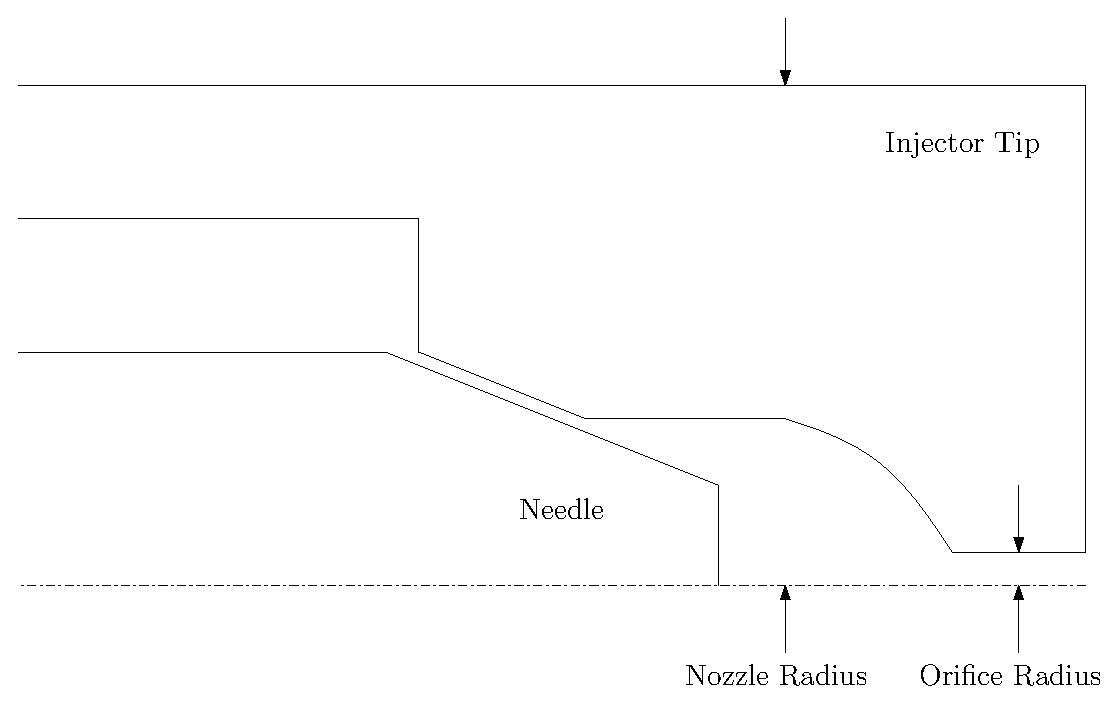
\includegraphics[width=0.4\textwidth]{nozzle.eps} \label{fig:nozzle}}
\subfigure[Represented injector tip]{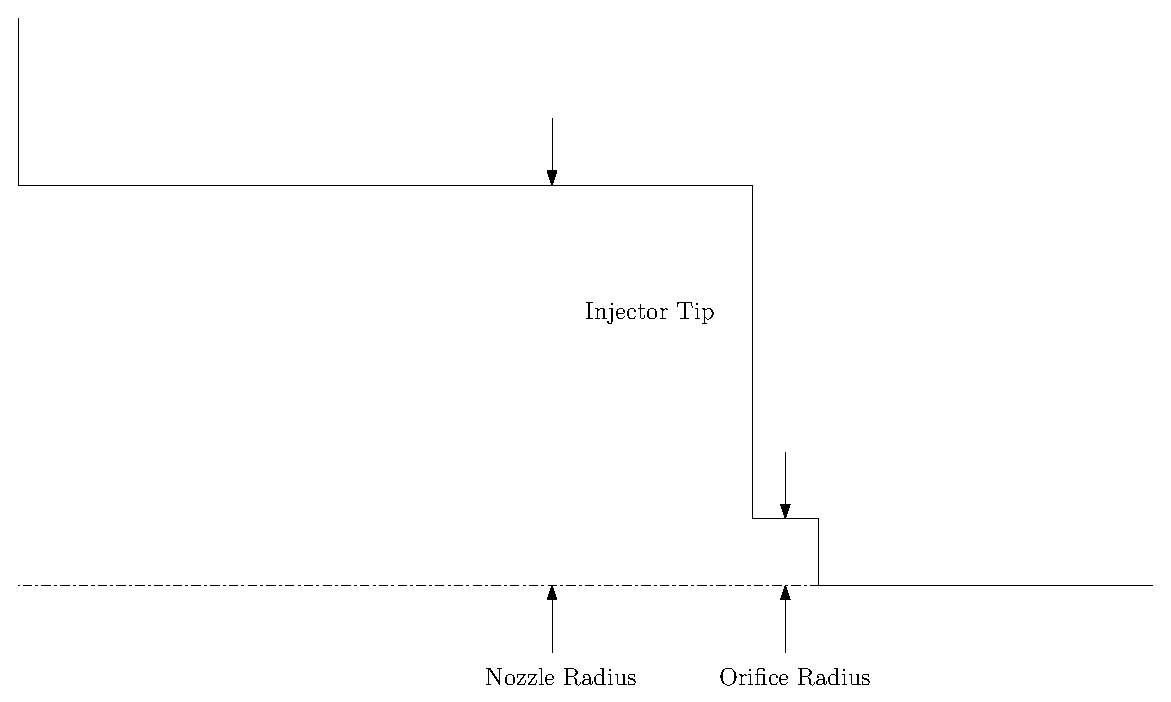
\includegraphics[width=0.4\textwidth]{nozzle_mod.eps} \label{fig:nozzle_mod}}
\caption{Schematics of the spray injector}
\end{figure}



\subsection{Injected Moments}
Moments of the injected droplet size distribution are based on the Gamma distribution \cite{yue2004}. Specifying three parameters: the liquid volume fraction, $\Theta$, Sauter mean radius, $r_{32}$ and the skewness parameter, $k$, the first two parameters $\mu_3$ and $\mu_2$ are found by
\begin{eqnarray}
\mu_3 &=& \frac{\Theta}{\frac{4}{3}\pi} \\
\mu_2 &=& \frac{\mu_3}{r_{32}}
\end{eqnarray}
and all other moments are determined recursively using the relation
\begin{equation}
\frac{\mu_{i+1}}{\mu_i} = r_{32} \frac{k+i}{k+2}
\end{equation}
The three parameters are related to the nozzle orifice radius, the injector operating conditions and how the nozzle orifice is modelled. Since the nozzle orifice is resolved, the exiting liquid volume fraction will be high ($0.9 - 1$). Such a high volume fraction is inconsistent with the assumption that the liquid is in the form of spherical droplets, though for the sake of resolving the injector and maintaining a simple injection model, this inconsistency is not rectified in this work.

The exiting bulk liquid is assumed to have been broken up into droplets, so the Sauter mean radius is approximated to be in the range $0.05r_{orif} - 0.15r_{orif}$. Finally, because only break-up of bulk liquid has taken place, the relative number of smaller droplets (than the mean) will be low, implying that the distribution will only have a weak positive skew, leading to a range of $3 - 7$ for parameter $k$.% (Fig. \ref{fig:gamma}).
% \begin{figure}[htp]
% \centering
% \includegraphics[width=0.6\textwidth]{gamma2.eps}
% \caption{Inlet PDFs with $r_{32}=1$ and $k=1.5,\; 2.25,\; 3,\; 7$ and  $14$.}
% \label{fig:gamma}
% \end{figure}



\subsection{Injection Velocity}
From the ambient pressure and the operating pressure of the injector, the average speed of the exiting liquid and entrained gas can be approximated by
\begin{equation}
U = C_d\,\sqrt{\frac{2(P_{inj}-P_{amb})}{\rho_d}}
\end{equation}
where the discharge coefficient, $C_d$, is approximately 0.7. The spray half-cone angle is then used to obtain the orifice outermost velocity. The variation of velocity towards the axis is controlled by an appropriate radial profile.



% \subsection{Radial Profiles}
% To reasonably approximate the behaviour of the exiting spray, the nozzle orifice face is discretized into a number of faces (typically 2 - 5), allowing the injector conditions to be varied radially (Fig. \ref{fig:orifice_mod}).
% \begin{figure}[H]
% \centering
% \includegraphics[width=0.49\textwidth]{orifice_mod.eps}
% \caption{Modelling of the nozzle orifice}
% \label{fig:orifice_mod}
% \end{figure}
% Radial profiles presented here are used for both the moments and the exiting injector speed (Fig. \ref{fig:radial_pr}). These profiles enable the representation of the higher concentration of the liquid towards the outer edge of the orifice (Fig. \ref{fig:radial_pr}$(a)$) due to swirl and the spread of the spray defined by the half-cone angle, applied to the speed (Fig. \ref{fig:radial_pr}$(b)$). The functions are defined as
% \begin{eqnarray}
% p_1(r)&=&\left(\frac{1}{r_{orif}}\,r\right)^{\beta_1} \\
% p_2(r)&=&\left(\frac{1}{r_{orif}}\,r\right)^{\beta_2}
% \end{eqnarray}
% for the moments and speed variation respectively, where $\beta_2<\beta_1<1$. Currently $\beta_1$ is set as 0.7 and $\beta_2$ as 0.3.
% \begin{figure}[H]
% \centering
% \includegraphics[width=0.49\textwidth]{radial.eps}
% \caption{Nozzle radial profiles}
% \label{fig:radial_pr}
% \end{figure}



% \subsection{Discharge Profiles}
% Two profiles are used to govern the discharge of the liquid from the injector (Fig. \ref{fig:discharge_pr}), where $t_1-t_0$ is the injection duration. The first profile (Fig. \ref{fig:discharge_pr}$(a)$) controls the quantity discharged, and the second profile (Fig. \ref{fig:discharge_pr}$(b)$) controls the rate of discharge. The rate of discharge profile, $p_2(t)$, extends beyond the liquid discharge profile, $p_1(t)$, to represent the pressure potential remaining constant throughout the duration of the discharge.
% \begin{figure}[H]
% \centering
% \includegraphics[width=0.49\textwidth]{discharge.eps}
% \caption{Nozzle discharge profiles}
% \label{fig:discharge_pr}
% \end{figure}



%%%%%%%%%%%%%%%%%%%%%%%%%%%%%%%%%%%%%%%%%%%%%%%%%%%%%%%%%%%%%%%%%%%%%%%%%%%%%%%
\section{Impaction Conditions} \label{sec:impac_cond}
Wall boundary conditions are based on the spray impingement model of \cite{bai1995}, where the condition of the wall and the state of the impinging spray determine the outcomes. If the wall is dry the velocity and moments of the splashing droplets are determined.  If the wall is wet, rebounding conditions in addition to splashing conditions are defined. An alternative model is described by \cite{grover2001} though is not considered here.

At the wall face (Fig. \ref{fig:wall}), the splashing and rebounding conditions are determined from the near-wall control volume injected spray state. The impacting spray boundary conditions at the wall are defined as being permeable, i.e. the spray passes through the wall. This prevents a build-up of moments in the near-wall control volume. To represent the build-up of liquid which actually would occur, the sum of the $\mu_3$ fluxes at the wall (multiplied by $\frac{4}{3}\pi$) becomes the source term for the liquid film equation.
\begin{figure}[htp]
\centering
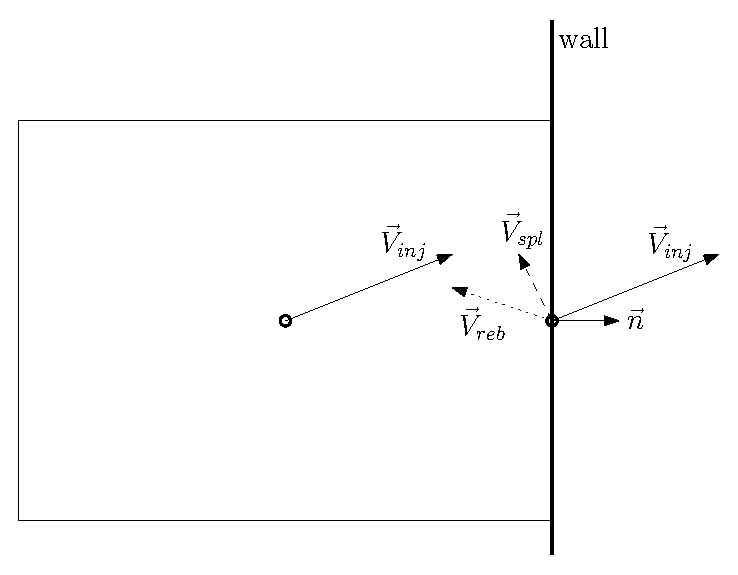
\includegraphics[width=0.49\textwidth]{wall.eps}
\caption{Division of the spray into injected, splashing and rebounding sprays}
\label{fig:wall}
\end{figure}



\subsection{Critical Radii}
In order to determine which droplets undergo the different processes, critical radii are obtained from the following correlations. Splashing and rebounding moments are calculated from integrating the near-wall PDF of the incoming spray between the limits prescribed by the critical radii. Moment-averaged splashing and rebounding velocities are calculated in a similar manner.



\subsubsection{Dry Walls}
Splashing takes place when
\begin{equation}
We_{d} La^{0.18} > C_{1,d}
\end{equation}
where $La$ is the Laplace number, defined as
\begin{equation}
La = \frac{2 \rho_d \sigma_d r}{\mu_d}
\end{equation}
$C_{1,d}$ is related to the wall roughness $r_s$ by
\begin{equation}
C_{1,d} \approx 2588 \,r_s^{-0.254}
\end{equation}
for wall roughness $0.05 \leq r_s \leq 12 \; \mu m$.



\subsubsection{Wet Walls}
Rebound takes place when
\begin{equation}
We_{d} < 5
\end{equation}
and splashing when
\begin{equation}
We_{d} La^{0.18} > 1320
\end{equation}
Droplets outside these ranges for both wet and dry walls are assumed to stick.  From these conditions, critical radii are determined and then used to integrate over the near-wall droplet distribution, obtaining the appropriate boundary condition moments for the splashing and rebounding spray.
A droplet undergoing splashing is assumed to break up into $N_{spl}$ droplets (taken as equal to 2 by \cite{lemini2002}), resulting in
\begin{equation}
\mu_{i} = N_{spl}^{\frac{3-i}{i}} \, \mu_{i,spl}.
\end{equation}



\subsubsection{Transition}
In practice, the wall becomes wet over the duration of the spray impacting on the wall.  This transition should be considered rather than assuming that either the wall is wet or dry from the outset.  To perform this transition, the method proposed here compares the volume fraction of the liquid film on the wall with a critical film volume fraction, $\theta_{wet}$, to determine whether the wall is wet.  If the volume fraction is less than the critical value and non-zero, the coefficient $C_{1,d}$ is modified by the function
\begin{equation}
C_{1,d}=\frac{1320-C_{1,d}}{\theta_{wet}} \, \theta + C_{1,d}
\end{equation}
and the wall is assumed to be dry.  The critical film volume fraction is taken as 0.01.



\subsection{Resultant Velocities}
Corresponding droplet velocities are calculated from the volume-averaged incoming velocity and the wall normal vector.
\begin{eqnarray}
\vec{v}_{in} &=& \vec{v}_{d}(r) \label{eqn:vel_in}\\
\vec{v}_{n} &=& \left( \vec{v}_{in} \cdot \vec{n} \right) \vec{n} \\
\vec{v}_{t} &=& \vec{v}_{in} - \vec{v}_{n} \\
\vec{v}_{out} &=& -C_{n} \vec{v}_{n} +C_{t} \vec{v}_{t}
\end{eqnarray}
For rebounding droplets, the process is assumed to be inelastic, resulting in the coefficients taking
\begin{eqnarray}
C_{n} &=& 0.993-1.76\theta+1.56\theta^{2}-0.49\theta^{3} \\
C_{t} &=& 0.714
\end{eqnarray}
where $ \theta $ is the incidence angle.  Splashing droplets take identical coefficients of 0.25 \cite{lemini2002}.

Upon integrating between the limits for the splashing and rebounding conditions, two set of moments and moment-averaged velocities will be obtained (for splashing spray and the rebounding spray). The likelihood is that within either set, the moment-averaged velocities will be dissimilar (assuming a non-uniform droplet velocity profile), potentially becoming a source of divergence for the model. To overcome this, the fourth moment-averaged velocities ($\vec{V}_{d,3,spl}$ and $\vec{V}_{d,3,reb}$) are used for all moments within their respective sets.



%%%%%%%%%%%%%%%%%%%%%%%%%%%%%%%%%%%%%%%%%%%%%%%%%%%%%%%%%%%%%%%%%%%%%%%%%%%%%%%
\section{Spray Model Parameters} \label{sec:model_param}
There are a number of parameters and submodels to choose from in order to define the complete spray model. This section is presented in order to show how the different parameters and submodels effect the overall spray and to come to conclusions about which parameters and submodels are most suitable.

The suitability of the choice of parameters and submodels is defined by meeting two conditions. First, that with a given configuration, the complete spray model remains stable throughout the entire simulation, and secondly, the Sauter mean radius (SMR) is physically sensible in all regions of the spray.

The range of parameters and submodels are listed in Table \ref{tab:spr_param}, where the initial reference parameters (and submodels) are shown in bold font and ideal parameters are marked by an asterisk. After a parametric case is performed, reference parameters referring to that case may be modified, whereby the modified parameters are used for subsequent parametric cases.

The computational grid, fluid properties and other configuration details of the test cases are exactly the same as those found in Sect. \ref{sec:wall_imp_case} detailing the wall impaction case.
%
\begin{table}[H]
% % \onehalfspacing
\caption{Parameters and submodels}
\vspace{2mm}
\centering
\begin{tabular}{l | l}
\hline \hline
Parameter/submodel & Options \\
\hline
Moments conv. bl. (HRIC) & \textbf{0}, 0.3, 0.6, 0.9 \\
Velocity conv. bl. (TVD: Min-mod) & \textbf{0}, 0.3, 0.6, 0.9 \\
\hline
Break-up model & RD, \textbf{PE}$^{\ast}$, HF \\
Velocity exponent, $b$ & 0.2, \textbf{0.4}, 0.6 \\
Collision model & \textbf{Off}, On$^{\ast}$ \\
\hline
SMR at injector, $r_{32,inj}$ ($\mu$m) & 15, \textbf{25}, 35 \\
Skewness of inj. PDF, $k_{inj}$ & 3, \textbf{7} \\
\hline
Temporal scheme & EI2, \textbf{EI3}$^{\ast}$ \\
Time step, $\Delta t$ ($\mu$s) & 1, \textbf{2}, 3$^{\ast}$ \\
\hline
Moments, $P_{\mu}[-]$ & $[1\,2\,3]$, $\mathbf{[2\,3\,4]}$, $[3\,4\,5]$, $[0\,1\,2\,3]$, ${[0\,1\,2\,3\,4]}^{\ast}$ \\
\end{tabular}
\label{tab:spr_param}
\end{table}

The overall shape of the spray is expected to be strongly effected by the accuracy at which the spray properties are convected and so the convection schemes are assessed first. Once the choice of blending for the moments and their momentums are decided, the break-up models are compared. As noted in the methodology, only the break-up model of \cite{pilch1987} (PE) covers all break-up regimes for any type of spray so is expected to be the model adopted. However, all three models are compared and are considered as suitable candidates. Velocity exponent is then varied to find out what degree of influence this has on the spray and then the collisions model is introduced.

Parameters of the injected distribution are not expected to have a strong effect on the overall spray. If the SMR is over-predicted, the break-up model should suitably reduce this and the collisions model is expected to compensate to some degree for an excessively positive-skew distribution. Here, this hypothesis is tested.

Comparison between the Euler implicit temporal discretization schemes is performed only to show whether adopting a three time levels method (EI3) makes any noticeable difference to the spray over the two time levels method (EI2). Very little difference, if any, is expected, since geometrical errors are expected to considerably out-weight temporal discretization errors, especially since the grid topology is non-orthogonal.

Convergence with a time step as large as 3$\mu$s is not expected, though is tested anyway. For the majority of cases found in \cite{beck2000}, the time step was set as 1$\mu$s. With improved temporal discretization (EI3), the possibility of using a larger time step is sought.

Finally, once all the major components of the spray model are set, the choice of transported moments is assessed. For the first three cases, the PDF will be reconstructed using the Gamma distribution, and for the last two cases, the Maximum Entropy method will be used as the primary choice and as the secondary choice the Gamma distribution will be used, based on the three highest order moments available ($[1\,2\,3]$ and $[2\,3\,4]$ respectively).

\textit{N.B.} All graphed SMR data presented is taken from the chordline of the spray as shown in Fig. \ref{fig:chord}.
\begin{figure}[H]
\centering
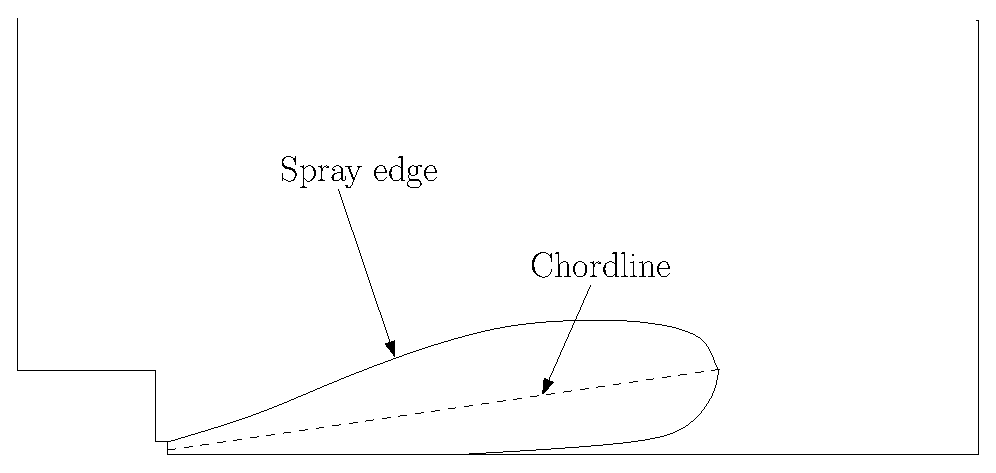
\includegraphics[width=0.49\textwidth]{chord.eps}
\caption{Chordline of the injected spray}
\label{fig:chord}
\end{figure}



\subsection{Number of Segments}
Before beginning the parametric cases, the number of segments required for the discretization of the PDF and droplet velocity profile is determined by plotting the cumulative inter-phase drag source term (since contributions to the source term are made over the entire droplet size range, unlike break-up and collision terms). Figure \ref{fig:n_seg} shows that whilst the cumulative term for the range of segmentations is almost identical (the source term can be calculated accurately with as few as 10 segmentations), the intermediate contributions converge with 40 segmentations.
\begin{figure}[H]
\centering
\label{fig:n_seg}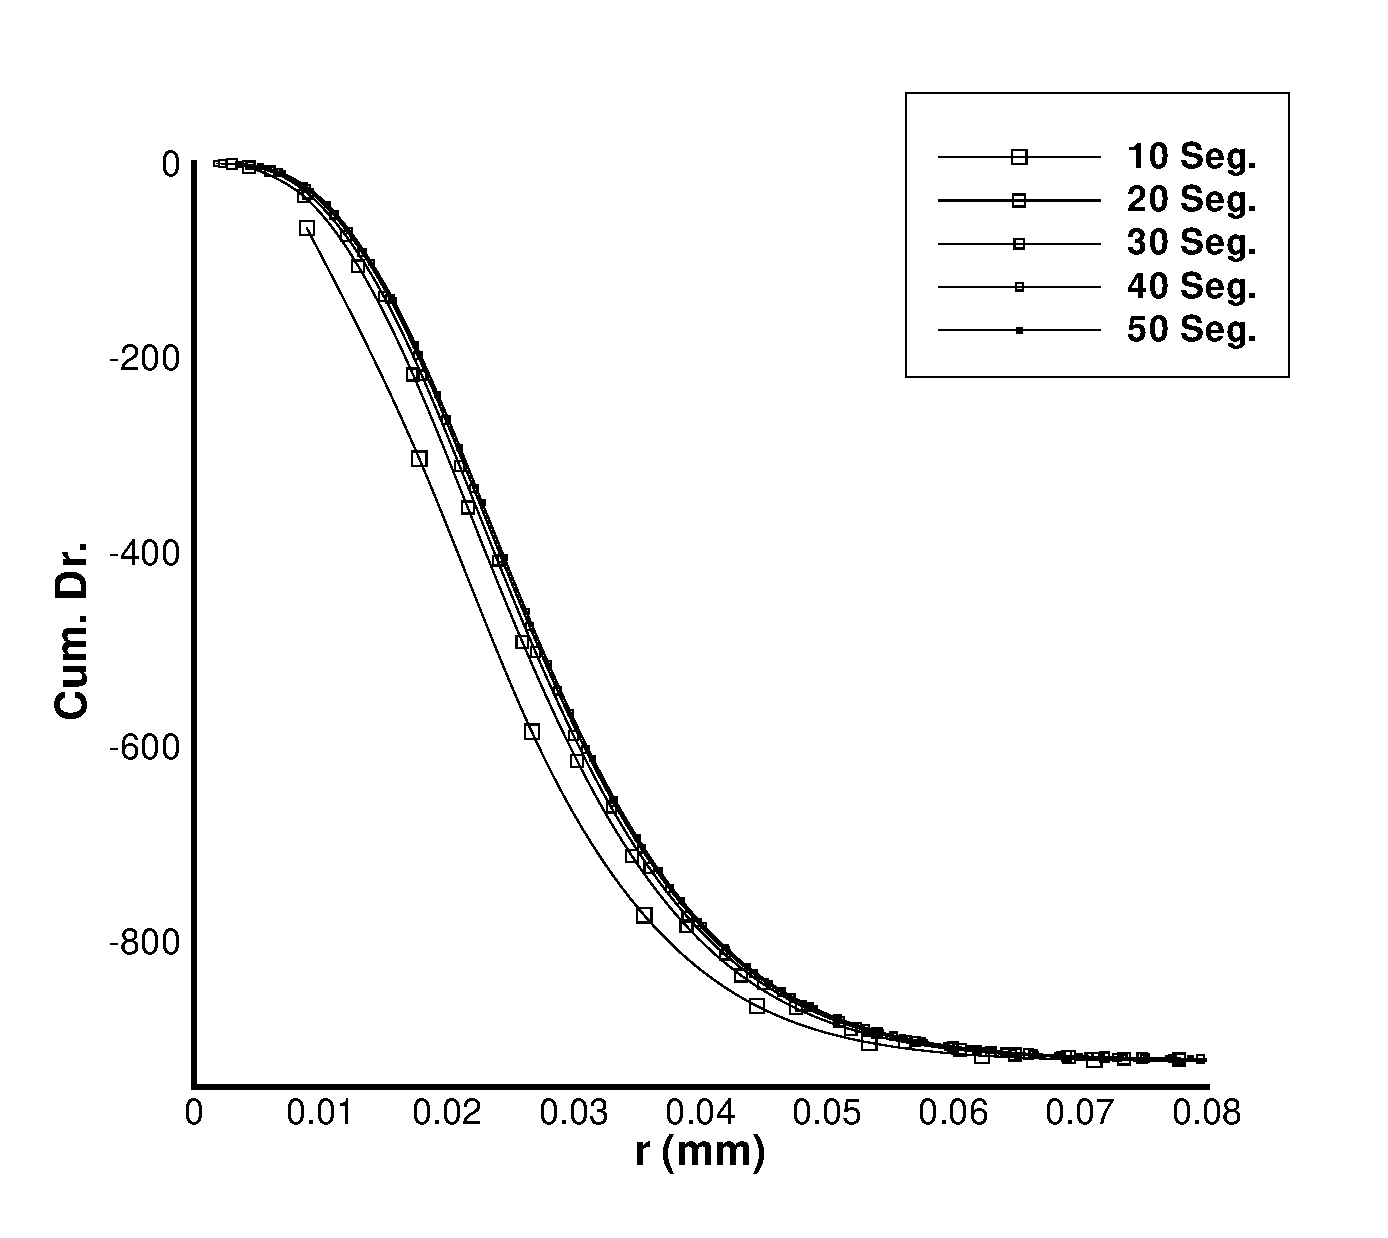
\includegraphics[width=0.49\textwidth]{n_seg.eps}
\caption{Convergence obtained for 40 segmentations}
\end{figure}
With 40 segmentations, the computational time required to solve the hydrodynamics was found to be disproportionate to the time required to solve the spray transport equations. As a result, the number of segmentations performed on the underlying distributions is reduced to 30.



\subsection{Convection Schemes} % pc_100
The testing of the convection schemes breaks down into two sections; first the spray alone is transported without spray hydrodynamics  activated (inter-phase drag and break-up) as a means of testing the boundedness of the transported moments for the various configurations. Once a suitable configuration is found, the hydrodynamics terms are activated and the spray model is tested with the optimal choice of convection schemes blending.

To determine whether the spray is being modelled in a bounded manner, the SMR is calculated. If the SMR deviates from the inlet SMR then the solution is not bounded. Both the min-mod total variation diminishing (TVD) scheme and the high resolution interface capturing (HRIC) scheme \cite{muzaferija1999} are blended with the implicitly implemented upwind differencing scheme (UDS). The degree to which the high order scheme is blended with the UDS scheme is listed in Table \ref{tab:spr_param}.

First, the calculated spray shape is shown in Fig. \ref{fig:uds} using UDS for both the moments and their momentum. This shows excessive false diffusion, as shown by the presence of the spray above the theoretical outer edge (determined from the injection angle) shown by the grey line cutting through the spray. SMR is constant throughout the spray.
\begin{figure}[H]
\centering
\includegraphics[width=0.49\textwidth]{pc_101.eps}
\caption{Spray shape with pure UDS}
\label{fig:uds}
\end{figure}

\subsubsection{Deferred Correction and Blending}
The method for implementing a higher order interpolation scheme to compute cell face fluxes ($F_k$) is to use the lower order scheme (UDS) to discretize the term to form the matrix entries and include the difference between the higher order scheme (HRIC or TVD) and the lower order scheme based on current values of the transported field in the right-hand side (the source term), as in
\begin{equation} \label{eqn:def_conv}
F_k = F_k^L + \gamma (F_k^H - F_k^L)^{curr}
\end{equation}
Normally, a value of $\gamma$ is set for each transport equation, typically in the range (0.5 - 1).

When solving the moment-averaged momentum equations using a high order convection scheme, it was found that augmentations to the source term by Eq. (\ref{eqn:def_conv}) must be zeroed where the spray does not exist, as shown in Fig. \ref{fig:zero_def_conv}. This step is essential for the spray to be transported using high-order convection schemes.
\begin{figure}[H]
\centering
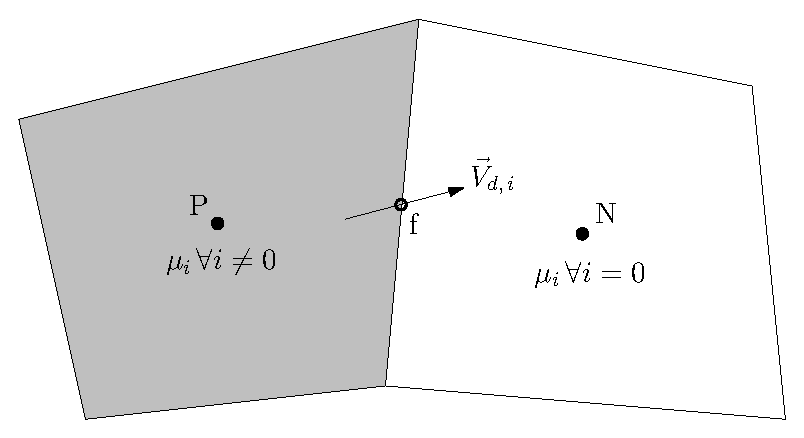
\includegraphics[width=0.49\textwidth]{vel_interp.eps}
\caption{$(F_k^H - F_k^L)^{curr}$ is set to zero in volume $\mathrm{N}$ since the spray is not present there.}
\label{fig:zero_def_conv}
\end{figure}



\subsubsection{Moments}
The effect of increasing the weighting of the HRIC on the moments is tested first (with UDS for momentum). From Fig. \ref{fig:hric} the trend shown is that increasing the weighting towards the HRIC scheme, the spray shape becomes more sharply defined, reducing false diffusion. The boundedness condition is perfectly satisfied, as shown in Fig. \ref{fig:hric_cl}.
\begin{figure}[H]
\centering
\subfigure[HRIC $\gamma=0.3$]{\includegraphics[width=0.32\textwidth]{pc_102.eps}}
\subfigure[HRIC $\gamma=0.6$]{\includegraphics[width=0.32\textwidth]{pc_103.eps}}
\subfigure[HRIC $\gamma=0.9$]{\includegraphics[width=0.32\textwidth]{pc_104.eps}}
\caption{Variation of spray shape due to HRIC interpolation}
\label{fig:hric}
\end{figure}
%
\begin{figure}[H]
\centering
\includegraphics[width=0.49\textwidth]{pc_103z.eps}
\caption{Radial diffusion along outer spray edge (HRIC $\gamma=0.6$)}
\label{fig:hric_103z}
\end{figure}
In addition to sharpening the spray shape, the penetration is reduced slightly with increasing $\gamma$, though there remains near-uniform radial diffusion along the outer edge of the spray which is present regardless of the value of the blending constant (Fig. \ref{fig:hric_103z}). This radial diffusion may be related to the manner in which interpolation is performed between radially adjacent CV convection coefficients (particularly $\mu_{i}$ in the flux term $\mu_{i}[\vec{V}_{d,i} \cdot \vec{n}]$ from Eq. (\ref{eqn:mome_eqn})). Further from the axis, volumetric values have greater influence so using linear interpolation (which does not account for volumetric change) will tend to exaggerate the influence of the CV values closer to the centreline, causing excess radial spread, as seen in Fig. \ref{fig:hric_103z}.
\begin{figure}[H]
\centering
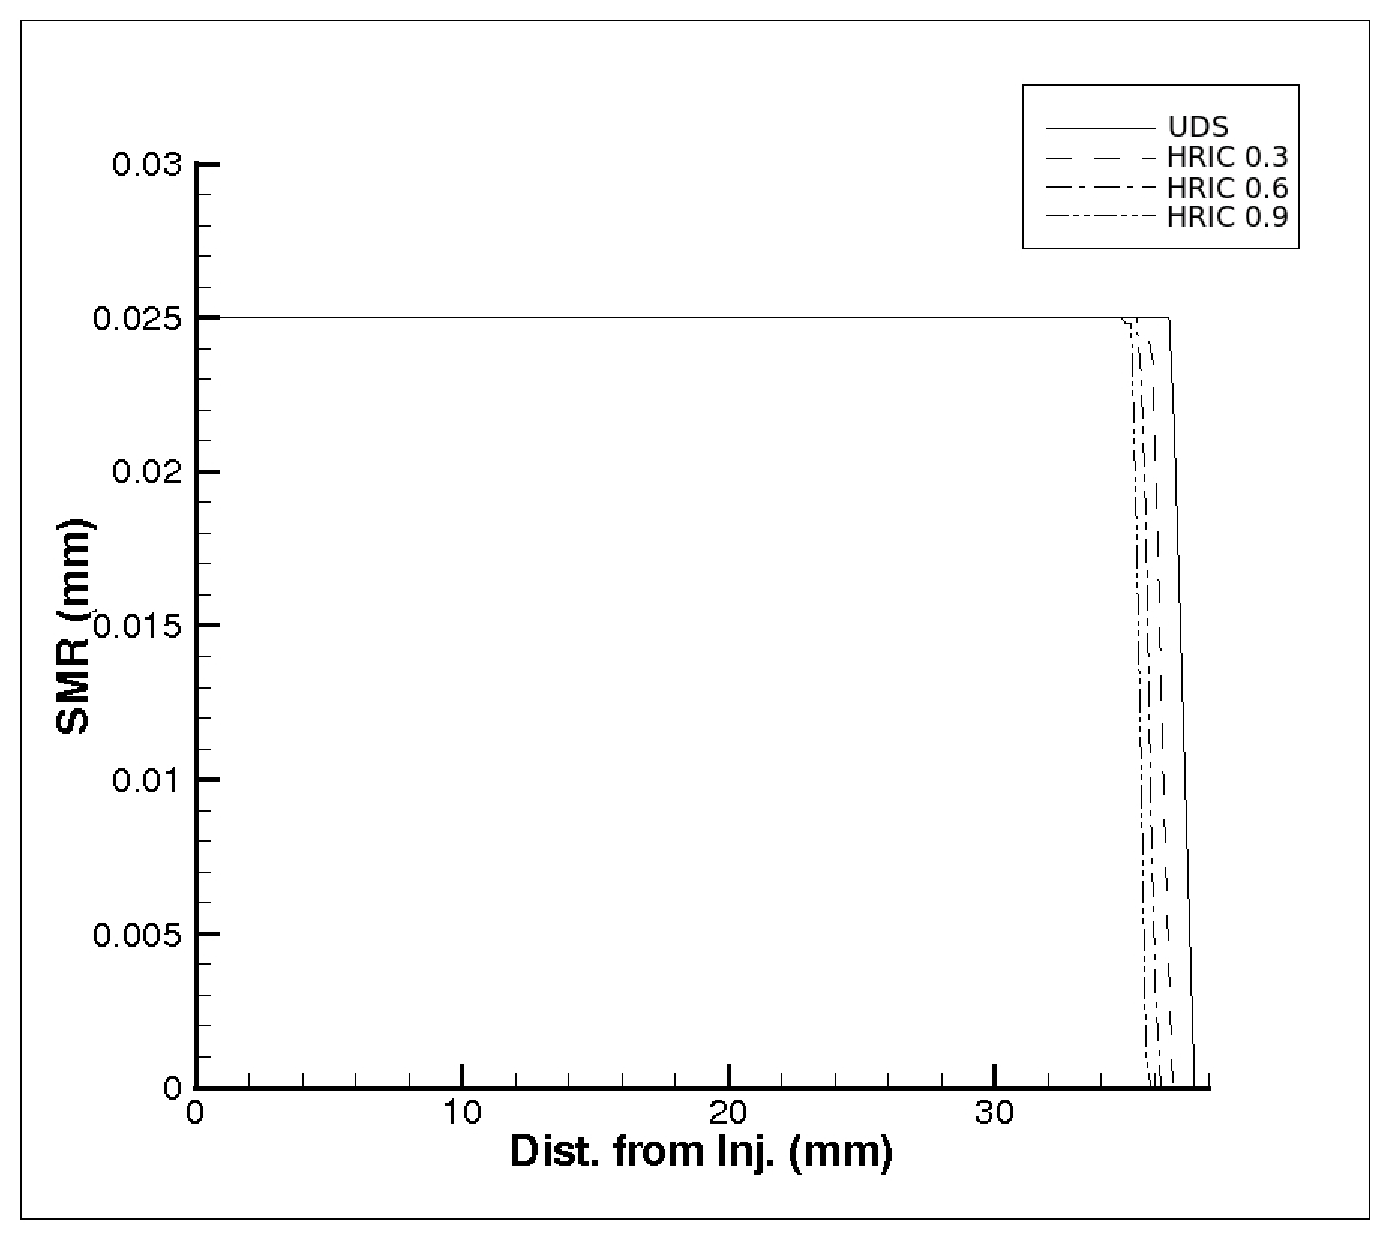
\includegraphics[width=0.49\textwidth]{pc_104_cl.eps}
\caption{Boundedness of spray using HRIC}
\label{fig:hric_cl}
\end{figure}



\subsubsection{Momentum}
The TVD scheme is the most appropriate higher order interpolation scheme to use for the momentum equations, since central differencing tends to cause unbounded solutions and HRIC is designed for resolving scalars (particularly concentrations). With the TVD scheme, a number of interpolation functions are available, but here only the Min-mod interpolation is tested (with UDS for the moments).

Sharpness of the spray shape is not effected by the increased weighting of the TVD scheme on the momentum (Fig. \ref{fig:tvd}), but the penetration is reduced to a much greater degree with the increased influence of the TVD scheme (Fig. \ref{fig:tvd_cl}) than compared with the previous case. Again the SMR is perfectly bounded.
\begin{figure}[H]
\centering
\subfigure[TVD: Min-mod $\gamma=0.3$]{\includegraphics[width=0.32\textwidth]{pc_105.eps}}
\subfigure[TVD: Min-mod $\gamma=0.6$]{\includegraphics[width=0.32\textwidth]{pc_106.eps}}
\subfigure[TVD: Min-mod $\gamma=0.9$]{\includegraphics[width=0.32\textwidth]{pc_107.eps}}
\caption{Variation of spray shape due to TVD interpolation}
\label{fig:tvd}
\end{figure}
%
\begin{figure}[H]
\centering
\includegraphics[width=0.5\textwidth]{pc_107_cl.eps}
\caption{Boundedness of spray using TVD}
\label{fig:tvd_cl}
\end{figure}



\subsubsection{Moments and Momentum}
Combining the blending of both the moments and their momentum, three further cases were performed (HRIC/TVD $\gamma=0.3$, HRIC/TVD $\gamma=0.6$ and HRIC/TVD $\gamma=0.9$). However, only the first case ran successfully and is documented below, in Fig. \ref{fig:hric_tvd}. There is no obvious reason why the second and third case failed to run properly since independently, both schemes have been shown to work, though it may be due to the difficulty in converging stiffer sets of the coupled moment and momentum equations. At 30\% blending, very little difference is found in the sharpening of the spray or its penetration compared to the pure UDS case.
\begin{figure}[H]
\centering
\subfigure{\includegraphics[width=0.49\textwidth]{pc_108.eps}}
\subfigure{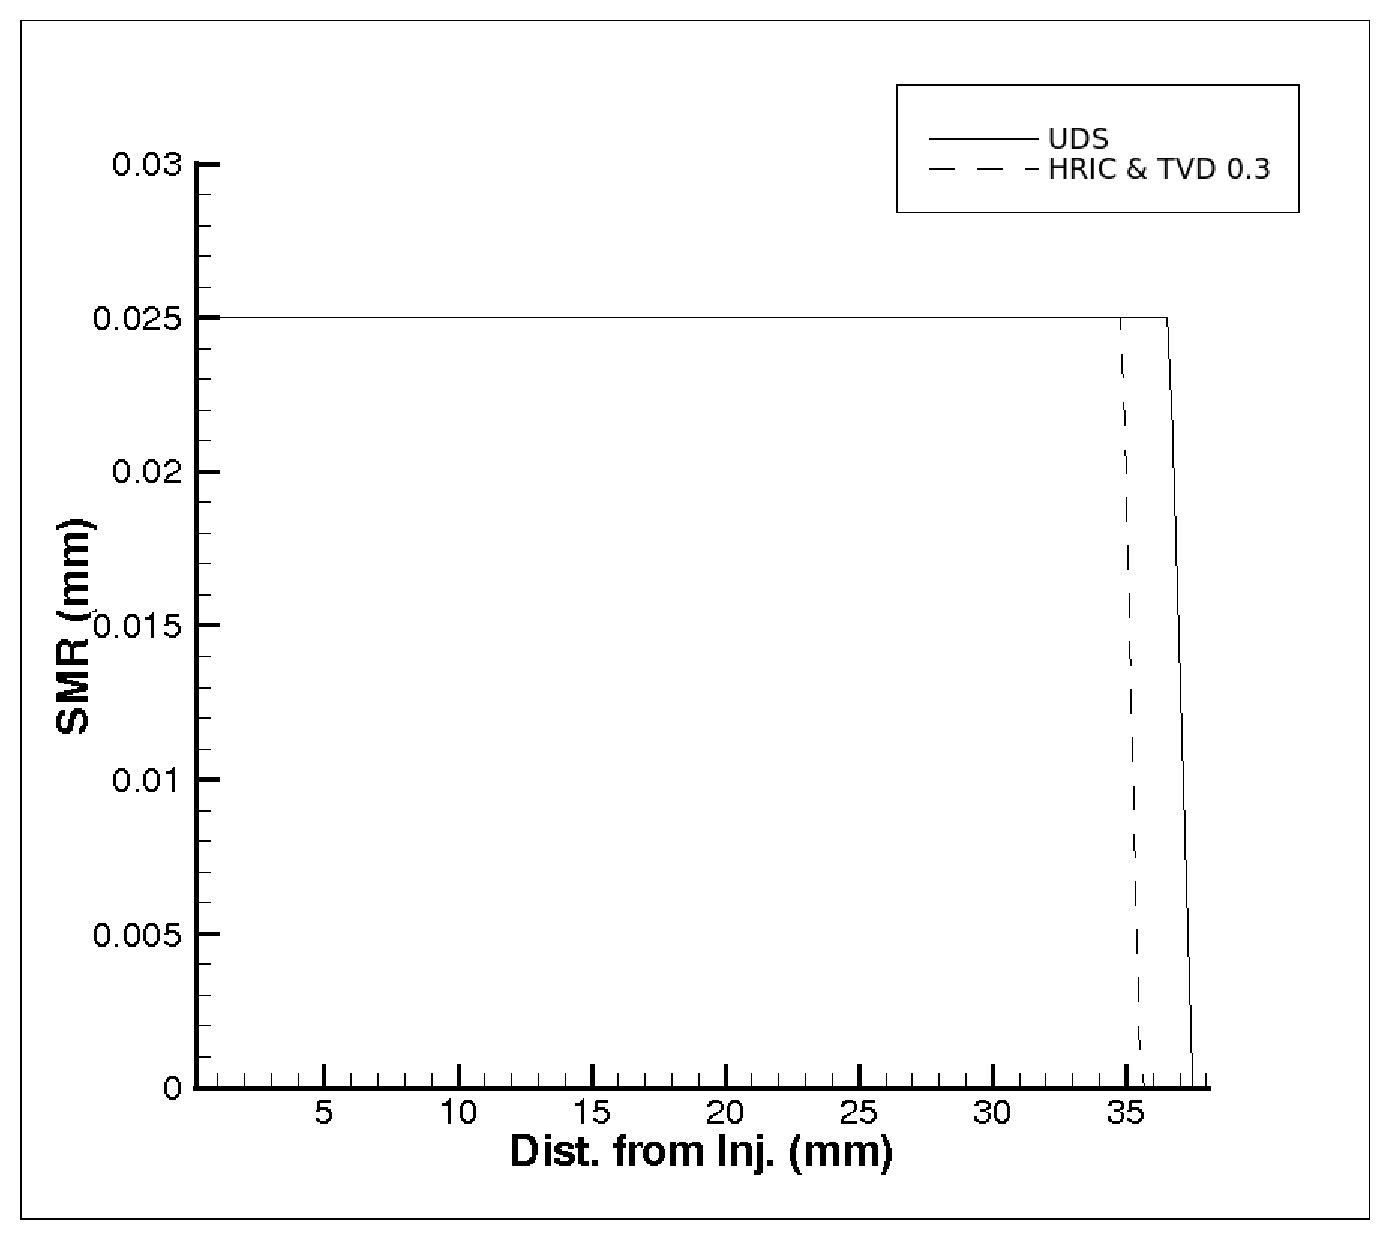
\includegraphics[width=0.49\textwidth]{pc_108_cl.eps}}
\caption{HRIC $\gamma=0.3$ and TVD: Min-mod $\gamma=0.3$}
\label{fig:hric_tvd}
\end{figure}



\subsubsection{Optimal Blending}
HRIC blending for the moments resulted in the greatest improvement in spray shape by reducing false diffusion, whereas using TVD for momentum, only the penetration was reduced. Combining the HRIC and TVD for the moments and momentum respectively caused the algorithm to become unstable for high degrees of blending.

For HRIC $\gamma=0.9$, false diffusion is minimized, maintaining a bounded solution so the reference blending parameters are revised to HRIC $\gamma=0.9$, TVD $\gamma=0$. With this condition implemented and the hydrodynamics activated, the spray model was run, though as shown in Fig. \ref{fig:hric_grph}, the SMR towards the spray tip was found to be unphysically large. Reducing the blending down to 0.6 presented a much more realistic droplet size variation.

The modification of the convection blending was not expected to have such as strong influence on the resulting SMR but only on the spray shape since its direct effect is only to cause higher concentrations in the spray by resolving its true edge more accurately. Figure \ref{fig:hric_grph} clearly shows, however, that the degree of blending has significant indirect influence, apparently presenting a choice between compromising on resolution of spray shape or on accuracy of the properties of the spray.

To simplify the problem, the reference break-up model (PE) was turned off and the HRIC $\gamma=0.6$ and HRIC $\gamma=0.9$ spray simulations were run again, leaving only in inter-phase drag model active. Figure \ref{fig:hric_grph} shows that without the break-up model on, the spray SMR for both cases are very similar, showing that the HRIC scheme is only influencing the spray shape, as expected, indicating that activation of the break-up model and variation of the HRIC blending somehow promotes a significant changes in the spray.

The prediction of the SMR becomes worse for larger values of $\gamma$ when the break-up model is active. Both the break-up source term and the HRIC scheme augment the right-hand side of the moments equations. When the break-up model is off, the moments equations are much less stiff than when break-up is on, making the equations much easier to converge, thus consistent behaviour is found (with regards to the SMR) for various values of $\gamma$ .

The normal way to treat stiff equations is to under-relax the solution scheme. However, the moments and momentum equations are already solved with relatively low under-relaxation factors (0.7 for all spray equations are used, whereas in \cite{beck2000} no  under-relaxation was performed). This apparently leaves no clear alternative than to make a compromise between spray shape accuracy and the accuracy of the SMR, thus the reference blending parameters are set to HRIC $\gamma=0.6$, TVD $\gamma=0$. To attempt to resolve the problem, the only clear way forward would be to revise the entire iterative solution scheme for solving the spray related transport equations, by introducing a robust predictor-corrector algorithm. This task however, is beyond the scope of the work.

\begin{figure}[H]
\centering
\includegraphics[width=0.49\textwidth]{pc_100_cl.eps}
\caption{Effect on the SMR by HRIC and break-up}
\label{fig:hric_grph}
\end{figure}



\subsection{Break-up Models} % pc_200
Droplet break-up is shown to have a significant effect upon the spray, as shown in Fig. \ref{fig:bre_pe} - \ref{fig:bre_cl}. From the comparison of the effects on the SMR by the models, two are found to be unsuitable; the models of \cite{hsiang1992} (HF) and \cite{reitz1986} (RD). These models excessively break up droplets, resulting in a large increase in the lower moments (momentarily reducing the SMR) which causes a rapid increase in drag for their corresponding velocities (particularly the lower moment-averaged ones), leading to very large SMR at the leading edge of the spray. Only the model of \cite{pilch1987} (PE) performs reasonably well, producing large SMR at the front end, but not to excess (Fig. \ref{fig:bre_pe}).  This break-up model is now set as the revised break-up option.

The reason why two of the models appear to perform poorly is not because of the models themselves but rather that those two models are only suitable for secondary break-up processes, where primary break-up is assumed to already have taken place. The spray model is not implemented with such a condition assumed. The model of \cite{pilch1987} compensates for this since it deals with the break-up of both primary and secondary droplets and is set as the revised parameter for this case.

\begin{figure}[H]
\centering
\subfigure[Effect of break-up using PE model]{\includegraphics[width=0.49\textwidth]{pc_202_p6.eps}\label{fig:bre_pe}}
\subfigure[Comparison of break-up models]{\includegraphics[width=0.49\textwidth]{pc_200_cl.eps}\label{fig:bre_cl}}
\caption{Effect of break-up models}
\label{fig:bre_ch}
\end{figure}



\subsection{Velocity Exponent} % pc_300
Data from three points within the spray are taken: the first is close to the injector (Point 1), the second is in the middle of the spray body (Point 2) and the last is close to the inside edge of the spray (Point 3). The extracted point data (the moments, continuum velocity and moment-averaged velocities) is shown in Table \ref{tab:point_data}, with the corresponding PDFs at each point shown in Fig. \ref{fig:d_pdf}.
%
\begin{table}[H]
% \onehalfspacing
\caption{Extracted data from the spray}
\vspace{2mm}
\centering
\begin{tabular}{| l | llll |}
\hline \hline
Point & $\mu_0$ (mm$^{-3}$) & $\mu_1$ (mm$^{-2}$) & $\mu_2$ (mm$^{-1}$) & $\mu_3$ \\
\hline
1 & 18467.9 & 169.204 & 2.03169 & 0.0294586 \\
2 & 6201.11 & 48.2283 & 0.482322 & 0.00561636 \\
3 & 684.43 & 0.894604 & 0.00125258 & 2.70287E-05 \\
\hline
\end{tabular}
\vspace{2mm}
\begin{tabular}{| l || l | llll |}
\hline \hline
Point & $v$ (m/s) & $V_{d,0}$ & $V_{d,1}$ & $V_{d,2}$ & $V_{d,3}$ \\
\hline
1 & 37.4231 & 101.471 & 102.005 & 102.318 & 102.437 \\
2 & 11.1468 & 74.447 & 68.5326 & 65.2815 & 67.5938 \\
3 & 1.2158 & 66.7343 & 57.5367 & 50.7085 & 58.2257 \\
\hline
\end{tabular}
\label{tab:point_data}
\end{table}
%
\begin{figure}[H]
\centering
\includegraphics[width=0.5\textwidth]{d_pdf.eps}
\label{fig:d_pdf}
\caption{PDFs from the extracted moments at points 1-3}
\end{figure}

The first method is presented in Fig. \ref{fig:d_m1} at points 1-3 for a range of exponent values (0.2, 0.4 and 0.6).  The index $i$ in Eq. (\ref{eqn:velocity_profile_exp}) is set as $3$. At points 1 and 2, very similar shaped velocity profiles are found since the underlying PDFs are similar and the difference between the continuum and spray velocity at both points is also similar. For the third point, where the underlying PDF has strong positive skew, the droplet velocity picks up slower for the small droplets compared with the droplet velocities at points 1 and 2. For large exponents ($b\geq0.4$) the velocity profile shows exaggerated values for the larger droplet size range compared with the corresponding moment-averaged velocities listed in Table \ref{tab:point_data}.
%
\begin{figure}[H]
\centering
\subfigure[Point 1]{\label{fig:d_p1m1}\includegraphics[width=0.32\textwidth]{d_p1m1.eps}}
\subfigure[Point 2]{\label{fig:d_p2m1}\includegraphics[width=0.32\textwidth]{d_p2m1.eps}}
\subfigure[Point 3]{\label{fig:d_p3m1}\includegraphics[width=0.32\textwidth]{d_p3m1.eps}}
\caption{Droplet velocity profile based on the exponential function}
\label{fig:d_m1}
\end{figure}


The exponential function has one free parameter, the exponent, $b$. To obtain a uniform distribution $b=0$, and for a linear distribution, $b=1$. Within that range, values for the exponent are considered. Before numerical tests on the spray are performed, 
the behaviour of the profile is assessed based on point data from \cite{jones2011}, along with its influence on the spray hydrodynamics models.

the effect on break-up, collision and inter-phase drag models are assessed based on data at point 1 (Table \ref{tab:point_data}), whereby the source terms relate to $\mu_0$ for break-up and collisions and $V_{d,0}$ and $V_{d,3}$ for inter-phase drag.

The effect of varying exponent $b$ on the hydrodynamic terms are shown in Fig. \ref{fig:s_p1m1} for break-up and collisions and Fig. \ref{fig:s_p1m1drg} for inter-phase drag.

\begin{figure}[H]
\centering
\subfigure[Velocity exponent, $b=0.2$]{\label{fig:s_p1m1v1}\includegraphics[width=0.32\textwidth]{s_v1.eps}}
\subfigure[Velocity exponent, $b=0.4$]{\label{fig:s_p1m1v2}\includegraphics[width=0.32\textwidth]{s_v2.eps}}
\subfigure[Velocity exponent, $b=0.6$]{\label{fig:s_p1m1v3}\includegraphics[width=0.32\textwidth]{s_v3.eps}}
\caption{Cumulative break-up model terms and collision term at point 1}
\label{fig:s_p1m1}
\end{figure}

Of the three break-up models, HF shows virtually no change in value for the range of exponents tested, whereas both RD and PE (the selected model) do. The influence on the collision source is minimal. Comparison between the change in drag due to variation of the exponent for both the first and fourth moment highlight how spray edge SMR can be controlled to a degree. The drag source term for $V_{d,3}$ is virtually unaffected by variation in $b$, unlike the drag source term for $V_{d,0}$ where the magnitude is significantly reduced when the exponent is increased from 0.2 to 0.6, enabling the lower moments to convect more readily, reducing the likelihood of producing exaggerated SMR.

\begin{figure}[H]
\centering
\subfigure[Drag term for $V_{d,0}$]{\label{fig:s_p1m1drg0}\includegraphics[width=0.32\textwidth]{s_drg0.eps}}
\subfigure[Drag term for $V_{d,3}$]{\label{fig:s_p1m1drg3}\includegraphics[width=0.32\textwidth]{s_drg3.eps}}
\caption{Cumulative drag terms at point 1}
\label{fig:s_p1m1drg}
\end{figure}

With exponents of 0.2 and 0.4, over-prediction of the leading edge SMR was found (Fig. \ref{fig:vel_exp}). Only by further increasing this value to 0.6 did the SMR drop at the front end of the spray, as shown in Fig. \ref{fig:vel_exp_p6}, thus the reference exponent is modified to 0.6. Even with such a large exponent as 0.6, the leading edge SMR does eventually pick up once the spray becomes more developed, as documented in Sect. \ref{sec:wall_imp_case}.

An exponent of 0.6 tends to push up the velocity of the larger droplets beyond what is sensibly expected. Consider the data at point 1 in Table \ref{tab:point_data}; the moment-averaged velocities are all around 102m/s, though Fig. \ref{fig:d_p1m1} shows the constructed droplet velocity range between 40 and 160m/s, whereby the lower bound is dictated by the continuum velocity. Clearly, 160m/s is well beyond the range of the moment-averaged velocities indicating unrealistic modelling of the droplet velocities. However, at present this is the only working configuration and so it is used.

The effective upper limit of the velocity profile can be determined by looking at the associated cumulative source terms. Break-up, collision and drag models (in Fig. \ref{fig:s_p1m1} and Fig. \ref{fig:s_p1m1drg}) show effectively no further contribution after 0.03mm, which corresponds to approximately 140m/s, presenting a more realistic velocity range.

\begin{figure}[H]
\centering
\subfigure[Velocity exponent, $b=0.6$]{\includegraphics[width=0.49\textwidth]{pc_303.eps}\label{fig:vel_exp_p6}}
\subfigure[SMR for $b=0.2$, $0.4$ and $0.6$]{\includegraphics[width=0.49\textwidth]{pc_300_cl.eps}\label{fig:vel_exp}}
\caption{Variation of velocity exponent}
\label{fig:vel_exp_ch}
\end{figure}



\subsection{Collisions Model} % pc_400
The introduction of the collisions model is expected to have the opposite effect (to some degree) on the spray compared to the break-up model. When the model is active, smaller droplets are coalescing to form larger droplets resulting in a reduction in the lower moments, manifested by an increase in the SMR. This in turn will effect the drag terms, but not to the same degree that break-up does. This behaviour is shown in Fig. \ref{fig:coll_mod}, comparing the SMR with and without the collisions model activated.
\begin{figure}[H]
\centering
\subfigure{\includegraphics[width=0.49\textwidth]{pc_402.eps}}
\subfigure{\includegraphics[width=0.49\textwidth]{pc_400_cl.eps}}
\caption{Activation of the collision model}
\label{fig:coll_mod}
\end{figure}
From this stage the following cases include the collisions model.


\subsection{Injection Parameters} % pc_500 (r_32)  pc_600 (k)
As expected, neither modifying the injection SMR nor the skewness of the injected PDF had significant effect on the overall spray (Fig. \ref{fig:inj_cond}). The only noticeable difference was that penetration was slightly increased for $r_{32,inj}=15\mu$m. This is unusual since larger droplets retain their momentum more readily, generally causing greater penetration. This early spray development may be due to the break-up model (PE) having little effect on the spray with injection SMR of 15$\mu$m, whereas for larger injection SMRs (25 and 35$\mu$m) the break-up model becomes active, reducing the penetration.
\begin{figure}[H]
\centering
\subfigure[Variation of injection SMR]{\includegraphics[width=0.49\textwidth]{pc_500_cl.eps}}
\subfigure[Variation of injection skewness]{\includegraphics[width=0.49\textwidth]{pc_600_cl.eps}}
\caption{Variation of injection parameters}
\label{fig:inj_cond}
\end{figure}



\subsection{Temporal Discretization} % pc_700 and 800
Time step values are based around those used by \cite{beck2002}. With the implementation of second order temporal interpolation, larger time steps are tested. Stability of the algorithm will be reduced with the increase of the time step, though a maximum value at which the algorithm remains stable and gives accurate results is sought.

Variation in the time step (Fig. \ref{fig:time_step}) shows very little difference in both the penetration and SMR, though 2$\mu$s will still be used for the calculations. Greater difference is shown between the choice of scheme (Fig. \ref{fig:temp_sch}). The penetration is noticeably different, with the Three levels discretization causing a reduction. This shows that the revision of the temporal scheme has been worthwhile.
\begin{figure}[H]
\centering
\subfigure[Temporal scheme effect]{\includegraphics[width=0.49\textwidth]{pc_700_cl.eps}\label{fig:temp_sch}}
\subfigure[Time step effect]{\includegraphics[width=0.49\textwidth]{pc_800_cl.eps}\label{fig:time_step}}
\caption{Variation of temporal parameters}
\label{fig:temp_disc}
\end{figure}



\subsection{Moments} \label{ssec:moments} % pc_900
If the Gamma distribution is used as the method of recovering the droplet size distribution, only three consecutive moments are required. Whilst any starting index is possible, the range of starting indices is chosen such that the volumetric based moment, $\mu_3$, is always transported. This is done so volume fractions of both phases are solved explicitly, rather than being derived from the recovered distribution, thus volume and mass concentration are more assured. Alternatively, if the Maximum Entropy distribution is used, consecutive moments from $\mu_0$ must be transported. This means that at least four moments must be transported to include $\mu_3$. However, five moments must be transported to represent the main quantities used to represent a distribution (mean, variance, skewness and kurtosis).

Of the five cases listed in Table \ref{tab:spr_param}, the last two did not run to completion ($[0\,1\,2\,3]$ and ${[0\,1\,2\,3\,4]}$). The reason why comes to light when the first three cases are examined ($[1\,2\,3]$, $[2\,3\,4]$ and $[3\,4\,5]$). Of the first three cases (Fig. \ref{fig:mom_gam}) the last two show strong resemblance, whereas the first case shows a huge increase in SMR at the leading edge of the spray. This shows that as lower moments are transported, the accuracy of the model degrades. The droplet velocity profile has already been shown to have a significant effect on the lower moment drag terms (Fig. \ref{fig:s_p1m1drg}) whereas for higher moment velocities, the shape of the profile causes only minor differences in the inter-phase drag. Unless the droplet velocity profile is accurately represented, divergence between low order moments is likely to occur resulting in the over-estimation of SMR found in Fig. \ref{fig:mom_gam} and in the first two cases referred to above.

From the comparison of the first three cases, the reference transported moments are revised, becoming $\mu_3$, $\mu_4$ and $\mu_5$, based on the trend that the further away from low order moments, the more stable the algorithm will be.

\begin{figure}[H]
\centering
\includegraphics[width=0.49\textwidth]{pc_900_cl.eps}
\caption{Choice of moments for the Gamma distribution}
\label{fig:mom_gam}
\end{figure}



\subsection{Parameters}
The revised default parameters and submodels options are listed in Table \ref{tab:spr_param_final}. Of the nine parameters tested across their ranges (Table \ref{tab:spr_param}), varying four of them caused the spray model to diverge for some values (convection blending, break-up models, velocity exponent and moments). Of these four parameters, all of them are considered as key parameters in the spray model.

\begin{table}[H]
% % \onehalfspacing
\caption{Revised parameters and submodels}
\vspace{2mm}
\centering
\begin{tabular}{l | l}
\hline \hline
Parameter/submodel & Option \\
\hline
Moments conv. bl. (HRIC) &  0.6 \\
Velocity conv. bl. (TVD: Min-mod) &  0 \\
\hline
Break-up model & PE \\
velocity exponent, $b$ & 0.6 \\
Collision model & On \\
\hline
SMR at injector, $r_{32,inj}$ ($\mu$m) & 25 \\
Skewness of inj. PDF, $k_{inj}$ & 7 \\
\hline
Temporal sch. & EI3 \\
Time step, $\Delta t$ ($\mu$s) & 2 \\
\hline
moments, $P_{\mu}[-]$ & $[3\,4\,5]$ \\
\end{tabular}
\label{tab:spr_param_final}
\end{table}

From the list of revised parameters, a final case is run whereby the geometry is modified to allow the spray to propagate freely, and the runtime is extended to two milliseconds. This test aims to show whether the spray calculations remain stable over long durations and to show whether the SMR remains at a sensible level.

The grid used for this case is shown in Fig. \ref{fig:open_grid}.
\begin{figure}[H]
\centering
\includegraphics[width=0.49\textwidth]{grid_open.eps}
\caption{Computational domain for open-ended case (5271 CVs)}
\label{fig:open_grid}
\end{figure}
The results revealed that whilst the algorithm remained stable, by 1.4ms the SMR had grown at the leading edge of the spray by over an order of magnitude from the injection SMR of 25$\mu$m, as shown in Fig. \ref{fig:open_smr}.
\begin{figure}[H]
\centering
\subfigure{\includegraphics[width=0.49\textwidth]{smr.eps}}
\subfigure{\includegraphics[width=0.49\textwidth]{smr_cl.eps}}
\caption{Sauter mean radius at 1.4ms}
\label{fig:open_smr}
\end{figure}
From this open-ended spray case and from the set of parametric cases, a preliminary conclusion can be drawn about the state of the presented spray model: the spray model becomes increasingly less accurate as it propagates. For the wall impaction case, this is not a problem since the wall prevents the spray from propagating, though for many other cases where the spray is not restricted, at present the spray model is not capable of simulating these accurately.


%%%%%%%%%%%%%%%%%%%%%%%%%%%%%%%%%%%%%%%%%%%%%%%%%%%%%%%%%%%%%%%%%%%%%%%%%%%%%%%
\section{Wall Impacting Spray: Park, et al (2004)} \label{sec:wall_imp_case}
The experimental cases of \cite{park2004} were performed to present a simplified analysis of late injection stratified charge mode found in direct injection engines. The spray model developed in this work will be used to replicate one of the experimental cases computationally in order to assess its performance at both simulating the spray and modelling the spray interaction with a wall.



\subsection{Case Parameters}
\subsubsection{Geometry}
The computational grid (Fig. \ref{fig:park_grid}) is arranged such that the injector tip is situated 38mm in front of the wall on which the spray impacts. The narrow-cone pressure-swirl injector operating at 6.8MPa producing a nominal cone angle of 20 degrees is assumed here to have an orifice radius of 0.25mm. The injector tip is shown as a bluff-body in the bottom left-hand corner of the grid.
\begin{figure}[H]
\centering
\includegraphics[width=0.49\textwidth]{grid.eps}
\caption{Computational domain for wall impaction case (5103 CVs)}
\label{fig:park_grid}
\end{figure}
Grid refinement is shown around the injector forming five injector inlet faces (Fig. \ref{fig:park_inj}), along the line of symmetry. A relatively coarse layer of cells is found along the right hand side of the grid, where the impacting wall boundary is defined (Fig. \ref{fig:park_wall}). This coarse layer is designed to avoid the liquid volume fraction in the near-wall cells becoming over-full. Finally, the protrusion at the top left hand corner of the grid is the outlet, situated far away from the spray. The outlet is necessary in this case since the flow is assumed to be incompressible.
\begin{figure}[H]
\centering
\subfigure{\includegraphics[width=0.49\textwidth]{grid_inj.eps}\label{fig:park_inj}}
\subfigure{\includegraphics[width=0.49\textwidth]{grid_wall.eps}\label{fig:park_wall}}
\caption{Injector and wall treatment}
\end{figure}
No grid independence testing is given here for two reasons. First, the grid presented is finer (in the areas of interest) than the grids used by \cite{beck2003,lemini2004}. In their grids, the injector was resolved with a maximum of three cells. Secondly, this is as fine a grid as can be afforded for this study, with the algorithm taking around 8 hours to complete (spray source terms plus twenty seven partial differential equations are solved per iteration).



% \subsubsection{Fluid Properties}
% The case is run at room temperature with an elevated pressure of 4.7kPa, giving a air density of 5.5kgm$^{-3}$. Molecular viscosity is taken as 1.846x10$^{-5}$kgm$^{-1}$s$^{-1}$. Iso-octane is the injected fuel, having a density of 702kgm$^{-3}$ and viscosity of 5.65x10$^{-5}$kgm$^{-1}$s$^{-1}$. Surface tension coefficient between air and Iso-octane is 0.0226kgs$^{-2}$.



% \subsubsection{Injector Conditions}
% Injected Sauter mean radius is set as one tenth of the injector orifice radius to 25$\mu$m and the skewness parameter $k=7$. Spray velocity and continuum velocity are assumed to be equal and are controlled by the discharge profile, $p_1(t)$, presented earlier. The profile is applied to both the velocities and the moments. Injection duration (pulse width) is set as 0.5ms with the rise time ($\delta t$ in Fig. \ref{fig:discharge_pr}$(a)$) set as 0.025ms. The rise time is an overestimate (it should be approximately 0.01ms), because divergence occurs if the injector is turned off too quickly.



\subsubsection{Modelling Parameters}
The case is run at room temperature with an elevated pressure of 4.7kPa, giving a air density of 5.5kgm$^{-3}$. Molecular viscosity is taken as 1.846x10$^{-5}$kgm$^{-1}$s$^{-1}$. Iso-octane is the injected fuel, having a density of 702kgm$^{-3}$ and viscosity of 5.65x10$^{-5}$kgm$^{-1}$s$^{-1}$. Surface tension coefficient between air and Iso-octane is 0.0226kgs$^{-2}$.

Injected Sauter mean radius is set as one tenth of the injector orifice radius to 25$\mu$m and the skewness parameter $k=7$. Spray velocity and continuum velocity are assumed to be equal. Injection duration is set as 0.5ms with the injector needle rise time set as 0.025ms. This rise time is an overestimate (it should be approximately 0.01ms), but is used because divergence occurs if the injector is turned on and off too abruptly.

Droplet velocity profile exponent is set to 0.6. Both the break-up model of \cite{pilch1987} [PE] and the collision model are employed. For determining whether the full set of moments are present in a given volume, the multiplier, $C_{\mu}$, is set to 1x10$^{-7}$. The underlying distribution is assumed to be a Gamma distribution and the moments $\mu_3$, $\mu_4$ and $\mu_5$ are used to determine its parameters. All terms related to the PDF and velocity profile are solved using numerical integration, discretized with 30 segments. Ideally the distributions should be divided into at least forty segments, though this is not done because of the computational cost incurred.



\subsubsection{Discretization}
Second order Euler implicit temporal discretization [EI3] is used for all transport equations, with a constant time step of 2$\mu$s. The convection discretization is detailed in table \ref{tab:desc_para}. No high order convection scheme is used for the moment-averaged momentum equation. Eddy viscosity is under-relaxed by the same constant used for the turbulence equations. Relatively low convection blending is used for the turbulence modelling to stabilize the algorithm.
\begin{table}[H]
% \onehalfspacing
\caption{Discretization Parameters for wall impaction case}
\vspace{2mm}
\centering
\begin{tabular}{l | c c}
\hline \hline
Transport equation & Under-relaxation & Convection blending \\
\hline
Continuum momentum & 0.7 & 0.9 (TVD: Min-mod) \\
Continuum turbulence & 0.65 & 0.5 (TVD: Min-mod) \\
Discrete momentum & 0.7 & 0 \\
Discrete continuity & 0.7 & 0.6 (HRIC) \\
\end{tabular}
\label{tab:desc_para}
\end{table}

Two iterations are performed on all gradient calculations, dropping the error one order of magnitude. Further iterations of the gradient showed very little gain in accuracy. Pressure and pressure correction are interpolated from the near-boundary CVs to the boundary after the first iteration.



\subsubsection{Initialization}
Only the turbulent kinetic energy and dissipation rate require non-zero domain initialization. Values of these are sought such that the resulting eddy viscosity is as small as possible without causing the algorithm to diverge early in the solution procedure. Over-estimation of eddy viscosity has been found to excessively resist the acceleration of the continuum phase.

The characteristic length scale of the initial turbulence is assumed to be 1cm with a velocity of 40m/s at 20\% intensity, giving initial eddy viscosity one hundred times greater than the molecular viscosity.



\subsubsection{Algorithm}
Outer iterations are limited to 20 and is assumed to converge once the global maximum normalized (1-norm) residual has dropped three orders of magnitude. Inner iterations (of the linear system) are required to drop the residual one order of magnitude.



\subsection{Penetration and Impaction}
Figure \ref{fig:park_spr} from \cite{park2004} shows the development and impaction of the spray, showing that impaction occurs at some time between 0.4 and 0.9ms. Cross-referencing this with the earliest recorded near-wall Weber numbers in Fig. \ref{fig:we_pre_ad} - \ref{fig:we_pre_cf}, impaction is most likely to have occurred around 0.9ms after the start of injection.
\begin{figure}[H]
\centering
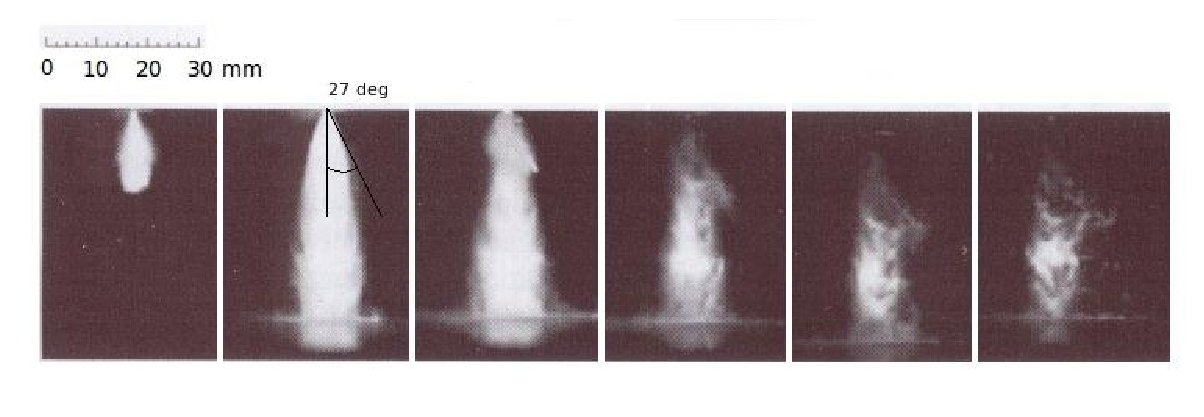
\includegraphics[width=0.99\textwidth]{fig4.eps}
\caption{Spray from 0.4ms at intervals of 0.5ms}
\label{fig:park_spr}
\end{figure}
From Fig. \ref{fig:park_spr} taken from \cite{park2004}, the spray half-cone angle is estimated as being 27 degrees. However, the cone angle is stated as being 20 degrees, implying a half-cone angle of 10 degrees. Clearly there is a discrepancy, so for the computational case a compromise is made by setting the half-cone angle to 20 degrees.

In the same figure, penetration at 0.4ms is shown to be approximately 16mm and at 0.9ms the spray reaches the wall, which is 38mm from the injector. This implies that the spray accelerates towards the wall, which is highly unlikely. A more likely explanation is that the first image in Fig. \ref{fig:park_spr} corresponds to an earlier time. Comparing the first two images in Fig. \ref{fig:park_spr} with the profiles in Fig. \ref{fig:smr_pre1}, good correlation of the spray shape is found at 0.9ms, especially at the front end of the spray. The experimental case shows a greater degree of spreading as the spray exits the nozzle, causing greater retardation to the spray than in the computational case.
\begin{figure}[H]
\centering
\subfigure{\includegraphics[width=0.49\textwidth]{smr_p4.eps}}
\subfigure{\includegraphics[width=0.49\textwidth]{smr_p9b.eps}}
\caption{Sauter mean radius at 0.4 and 0.9ms}
\label{fig:smr_pre1}
\end{figure}

Early spreading of the spray outwards is strongly resisted by the gas phase as it is drawn towards the injector orifice by the sharp drop in pressure in that region, forming a small vortex just in front of the nozzle (Fig. \ref{fig:inj_gas}).
\begin{figure}[H]
\centering
\includegraphics[width=0.49\textwidth]{inj_gas.eps}
\caption{Near-nozzle flow of the surrounding gas (at 0.4ms)}
\label{fig:inj_gas}
\end{figure}

The penetration rate of the spray model shown in Fig. \ref{fig:spr_pen} appears to be accurate, gradually slowing down as the spray progresses with spray tip arriving at the wall by 0.9ms, which is the initial impaction time recorded by \cite{park2004}.
\begin{figure}[H]
\centering
\includegraphics[width=0.49\textwidth]{pen.eps}
\caption{Penetration rate of the spray model}
\label{fig:spr_pen}
\end{figure}

Although the injector pulse width is only 0.5ms, at both 0.9 and 1.4ms there still appears in Fig. \ref{fig:park_spr} to be a strong concentration of the spray from the injector tip, appearing as though the injector is still spraying. This is also found in the computational results, as shown in Fig. \ref{fig:smr_pre1} - \ref{fig:smr_pre3}, but with a reduced spray width at the tail-end of the spray. (At 10mm from the injector at 0.9 and 1.4ms the spray width is 9mm and 8mm respectively, whereas the computational results show half-thicknesses of 3mm and 2mm, respectively.)
%
\begin{figure}[H]
\centering
\subfigure{\includegraphics[width=0.49\textwidth]{smr_1p4.eps}}
\subfigure{\includegraphics[width=0.49\textwidth]{smr_1p9b.eps}}
\caption{Sauter mean radius at 1.4 and 1.9ms}
\label{fig:smr_pre2}
\end{figure}

The contraction of the spray is attributed to the effect the continuum has on these trailing droplets. Figure \ref{fig:vort_gas} shows how the gas phase velocity forms an anti-clockwise vortex, which pushes the upstream spray towards the centreline resulting in a smaller SMR along the chordline (Fig. \ref{fig:smr_2p9_cl}) and pulls the downstream spray outwards.
\begin{figure}[H]
\centering
\subfigure[Anti-clockwise vortex formed in the gas phase (at 1.2ms)]{\includegraphics[width=0.49\textwidth]{vort_gas.eps}\label{fig:vort_gas}}
\subfigure[SMR along the chordline from 0.4ms to 1.4ms]{\includegraphics[width=0.49\textwidth]{smr_2p9_cl.eps}\label{fig:smr_2p9_cl}}
\caption{Effect of the gas flow on the spray}
\end{figure}

Only after 1.9ms does the spray concentration drop downstream of the injector. This pattern of the spray development indicates that the trailing edge of the spray after injection is completed is being carried by the surrounding gas. This retardation of the trailing edge of the spray was also found in the computational model, as shown in Fig. \ref{fig:smr_pre2} - \ref{fig:smr_pre3}.
\begin{figure}[H]
\centering
\subfigure{\includegraphics[width=0.49\textwidth]{smr_2p4.eps}}
\subfigure{\includegraphics[width=0.49\textwidth]{smr_2p9b.eps}}
\caption{Sauter mean radius at 2.4 and 2.9ms}
\label{fig:smr_pre3}
\end{figure}

Chordline values of volume weighted SMR show the drop in mean radius near the wall due to the break-up of splashing droplets. Further out from the wall the SMR picks up because the splashing droplet distribution is strongly positively skewed.
\begin{figure}[H]
\centering
\includegraphics[width=0.49\textwidth]{smr_2p9b_cl_fix.eps}
\caption{Sauter mean radius along the chordline from 1.9ms to 2.9ms}
\label{fig:smr_2p9b_cl}
\end{figure}



\subsection{Near-wall Weber Number}
The droplet Weber number
\begin{equation}
We_d = \frac{2r\,\rho_d V_{d,n}^2 }{\sigma_d}
\end{equation}
is sampled at locations in front of the wall, as shown in Fig. \ref{fig:park_we}. Line $abc$ is 1mm above the wall, line $def$ is 3mm above the wall and lines $ad$, $be$ and $cf$, are 0, 4 and 8mm from the centreline.
\begin{figure}[H]
\centering
\includegraphics[width=0.49\textwidth]{we_loc.eps}
\caption{Sampled Weber number locations}
\label{fig:park_we}
\end{figure}


Pre-impingement Weber numbers at each location were measured with respect to time and are plotted in Fig. \ref{fig:we_pre_ad} - \ref{fig:we_pre_cf}, showing both the experimental data and the computational data where the spray was present. In \cite{park2004} it is stated that the near-wall drop radii were in the range of 2 to 50 $\mu$m and the normal droplet velocity component was less than 15m/s. Computational data showed substantial over-prediction of the droplet velocity (with the largest value of 27m/s), which when squared in the calculation of the Weber number, further magnifies the error.

With the impinging droplets having such momentum, the post-impingement droplets will tend to have sufficient momentum to overcome the cross-flow of the gas phase, resulting in the droplets penetrating into the oncoming spray rather than being carried radially outward over the wall.
\begin{figure}[H]
\centering
\subfigure{\includegraphics[width=0.49\textwidth]{loc_a.eps}}
\subfigure{\includegraphics[width=0.49\textwidth]{loc_d.eps}}
\caption{Weber number before impaction at positions $(a)$ and $(d)$}
\label{fig:we_pre_ad}
\end{figure}

Since the spray form was assumed to be a hollow cone shape in the computation, no centreline data exists in front of the wall (Fig. \ref{fig:we_pre_ad}). However, experimental data shows a very clear presence of droplets heading towards the wall along the centreline. This indicates that the spray should have been modelled to consider the pre-swirl injection stage, as discussed in \cite{wigley2001} (though details about the transient behaviour of the process in this case are lacking), whereby fuel initially exits the nozzle along the centreline as the injector needle opens and develops into a hollow cone as the spray gains swirl momentum (Fig. \ref{fig:wigley}).
\begin{figure}[H]
\centering
\includegraphics[width=0.49\textwidth]{wigleyc.eps}
\caption{Pre-swirl injection stage \cite{wigley2001}}
\label{fig:wigley}
\end{figure}


Four millimetres out from the centreline, the difference between the spray and the computational model are shown in Fig. \ref{fig:we_pre_be}. Initial over-prediction of the Weber number does decay rapidly with time, though by 4ms the entire injected spray has interacted with the wall.
\begin{figure}[H]
\centering
\subfigure{\includegraphics[width=0.49\textwidth]{loc_b.eps}}
\subfigure{\includegraphics[width=0.49\textwidth]{loc_e.eps}}
\caption{Weber number before impaction at positions $(b)$ and $(e)$}
\label{fig:we_pre_be}
\end{figure}

At the outer edge of the spray, the Weber numbers of the computation model remain high, whereas the experimental data shows decaying Weber numbers away from the centreline.
\begin{figure}[H]
\centering
\subfigure{\includegraphics[width=0.49\textwidth]{loc_c.eps}}
\subfigure{\includegraphics[width=0.49\textwidth]{loc_f.eps}}
\caption{Weber number before impaction at positions $(c)$ and $(f)$}
\label{fig:we_pre_cf}
\end{figure}



Post-impingement Weber numbers are shown in Fig. \ref{fig:we_prepost}, where the experimental data is taken at the centreline position $(a)$ and the computational data is taken at position $(b)$ because no data exists for position $(a)$. The computational model shows that droplets rebound immediately after the spray begins to impact on the surface, whereas in the experimental case this only occurs after 3ms, implying that droplets prior to this time stuck to the surface, forming a film of liquid. Once the film is formed, rebounding readily occurs for droplets with low Weber numbers ($We<5$).
\begin{figure}[H]
\centering
\subfigure{\includegraphics[width=0.49\textwidth]{loc_b_post.eps}}
\caption{Weber number before and after impaction at position $(a)$}
\label{fig:we_prepost}
\end{figure}



\subsection{Wall Wetting}
The wetted patch from the experimental results has a radius of approximately 11mm, which compares reasonably well with the wetted footprint produced by the model, shown in Fig. \ref{fig:film}.
\begin{figure}[H]
\centering
\subfigure{\includegraphics[width=0.49\textwidth]{film.eps}}
\caption{Near-wall liquid volume fraction}
\label{fig:film}
\end{figure}



\subsection{Discussion}
The complete spray model operating with optimal parameters shows that the current implementation is capable of simulating spray propagation and wall interaction to a reasonable degree of accuracy. The poor accuracy found in the comparison of near-wall Weber numbers is likely to be associated with the parameters set for the injection conditions, particularly the half-cone angle.

Further simulations were run with wider half-cone angles (25 and 30 degrees) though neither case ran to completion due to numerical divergence after 0.7ms. The cause of divergence is likely to be related to the increased effect of drag on the spray causing greater differentiation of the moments, leading to over-estimation of the SMR. These tests were attempted based on the assumption that as the cone angle is increased, near-wall droplet velocity would drop, bringing the Weber numbers more in line with the experimental data.

Further experimental comparisons with the spray model are not documented in this section since the parametric tests earlier in this chapter showed that the model is still in a substandard condition. Until the problematic parametric cases are re-addressed and corrected and the model is shown to be robust, such comparisons are considered to be of limited use.


%%%%%%%%%%%%%%%%%%%%%%%%%%%%%%%%%%%%%%%%%%%%%%%%%%%%%%%%%%%%%%%%%%%%%%%%%%%%%%%
\section{Conclusion}
Despite the capacity that the Maximum Entropy formalism has for constructing accurate distributions, its incorporation into the spray model presented no benefit. This is not due to the method itself, but to the apparently divergent nature of the current formulation of the spray model.% It appears that the key detail to improve in the present model is the droplet velocity profile.

Although the revised droplet velocity profile did not characterize the droplet velocity accurately enough to allow the lower moments to be transported properly, it provides sufficient improvement to enable the full spray model to be run using high order moments. Varying the exponent showed how significantly the velocity distribution effects the characteristics of the spray, indicating how important it is to ensure the profile is estimated accurately.

% Further research is necessary for developing well behaved droplet velocity profiles based on the complete set of available moment averaged velocities.  General forms could be constructed using the methods presented for the construction of the probability density function.  An accurate representation of the droplet velocity is the key component to successfully implementing this spray model since it is required in all the source terms and boundary conditions presented.  As discussed by \cite{tagliani2001}, the reconstruction of such a distribution is well conditioned, so should not be too difficult to compute.

The hydrodynamic contributions are generally over-estimated for the lower order moments (such as the inter-phase drag) which is due to either the droplet size distribution being too strongly positively skewed and/or the droplet velocity profile over-estimating the difference between the velocity of the smaller droplets and the velocity of the surrounding gas. An attempt to minimize this difference could be performed by prescribing certain conditions of the velocity profile, such as its derivative must be equal to zero at the limits of the profile.

High order convection schemes for all transport equations were implemented. The lack of such schemes was a major shortcoming in both the works of \cite{beck2000} and \cite{lemini2004} and those authors acknowledged the need to address this. Two new schemes were implemented; the TVD scheme for the velocities and turbulence models and HRIC scheme for the moments. The use of the HRIC scheme had the most significant effect on the spray, enabling clearer resolution of the hollow cone spray structure. Implementation of the Three time levels method for approximating the temporal terms show noticeable, though not considerable, difference in the spray compared to the Euler implicit scheme used by \cite{beck2000}.

A suitable wall impaction model was implemented successfully to the spray model which retains as much detail of the rebounding and splashing sprays as the impinging spray, enabling coexistence of all three sprays within a given volume. The model has been shown to work successfully, transitioning the impaction conditions from dry to wet with the data obtained from the liquid film equation.

% When interpenetration of sprays occur, such as when the incoming and rebounding sprays cross paths near the wall, the current collision model does not consider collision between the two sprays. Extension of the collision model to consider this possibility is required.
% 
% When interpenetration of sprays occur, such as when the incoming and rebounding sprays cross paths near the wall, the current collision model does not consider collision between the two sprays. Extension of the collision model to consider this possibility is required.


%%%%%%%%%%%%%%%%%%%%%%%%%%%%%%%%%%%%%%%%%%%%%%%%%%%%%%%%%%%%%%%%%%%%%%%%%%%%%%%
\bibliographystyle{plain}
\bibliography{\REF references.bib}

\end{document}
